\documentclass{article}

\usepackage[utf8]{inputenc}
\usepackage[french]{babel}

\usepackage{lmodern}
\usepackage{graphicx}
\usepackage{hyperref}
\usepackage{graphicx}
\usepackage{natbib}
\usepackage{tcolorbox}
\usepackage{xcolor}
\usepackage{geometry}
\graphicspath{ {./res/} }

\definecolor{needcolor}{HTML}{007ACC}
\definecolor{nonfunctionnalneedcolor}{HTML}{9722ff}
\definecolor{subneedcolor}{HTML}{28A745}
\definecolor{duedateassigncolor}{HTML}{FF9800}

\tcbuselibrary{skins, breakable}
\newtcolorbox{needbox}[1][]{
  colframe=needcolor,
  colback=needcolor!10,
  coltitle=white,
  fonttitle=\bfseries,
  title=#1,
  breakable,
  enhanced,
  sharp corners=all
}

\newtcolorbox{nonfunctionnalneedbox}[1][]{
  colframe=nonfunctionnalneedcolor,
  colback=nonfunctionnalneedcolor!10,
  coltitle=white,
  fonttitle=\bfseries,
  title=#1,
  breakable,
  enhanced,
  sharp corners=all
}

\newtcolorbox{justificationbox}[1][]{
  colframe=subneedcolor,
  colback=subneedcolor!10,
  coltitle=white,
  fonttitle=\bfseries,
  title=#1,
  breakable,
  enhanced,
  sharp corners=all
}

\author{
    Valentin Jonquière,
    Mathilde Chollon,
    Denis Demirci,
    Iwen Jomaa,
    Jonathan Landry
}

\title{Rapport Final projet de programmation, Échecs en Java}

\begin{document}

\maketitle

\pagebreak

\tableofcontents

\pagebreak
\begin{abstract}
    Les images fournies dans le rapport sont parfois petites.
    Elles sont disponibles dans le dossier \textit{reports/final/res}
    sur notre repository GitLab.
 \end{abstract}

\section{Description de l'existant}
\subsection{Origine des Échecs}
Le jeu d’échecs, aussi appelé le jeu des Rois, est un jeu de stratégie dans lequel deux joueurs s’affrontent,
et le but est de faire échec et mat, c’est-à-dire arriver dans une position où il est possible de capturer
le Roi adverse et donc gagner la partie après n’importe quel coup joué par notre opposant (hormis capturer notre roi).
Le jeu d’échecs se joue sur un échiquier, un plateau de 8 lignes et 8 colonnes, 64 cases au total avec des pièces
caractérisées par certaines propriétés uniques. De manière compétitive, le jeu d'échecs effectue un classement
basé sur un système de points, appelés "Élos". Il sert à estimer le niveau d'un joueur (humain comme ordinateur) et
à répartir ces joueurs en catégories. Pour donner un ordre d'idée, le champion du monde possède un Élo aux alentours de 2900,
tandis qu'un joueur débutant qui connaît comment les pièces se déplacent est aux alentours des 400 Élos. Ce système d'Élo
va notamment nous permettre d'approximer le niveau de notre Intelligence Artificielle développée dans le cadre de ce projet.\\
Les origines de ce jeu restent méconnues, mais la légende la plus célèbre raconte que le précepteur d’un jeune prince en Inde
voulait simplifier les mécanismes de la société et inventa ainsi un échiquier avec des pièces, chacune jouant un rôle précis,
avec le Roi, la pièce maîtresse. Le prince fut alors émerveillé et en gage de remerciements, il demanda à son précepteur ce
qu’il souhaitait avoir comme présent. Ce dernier répondit qu’il voulait 1 grain de riz sur la première case, 2 grains de riz
sur la deuxième, 4 grains de riz sur la troisième, etc. jusqu’à la dernière case. Sur la 64ème case, il avait donc
2 puissance 63 grains de riz, soit de quoi recouvrir le pays entier avec une couche de riz.

\subsection{Variantes du jeu d'échecs}
À travers les années, les échecs ont été popularisés et ont donné naissance à de nombreuses variantes. Parmi les plus connues, on trouve :
\begin{itemize}
    \item Les échecs aléatoires de Fischer (Chess960) : Une variante inventée en 1996 par Bobby Fischer où la position initiale des pièces est aléatoire
    (mais reste miroir, c'est-à-dire que les blancs et les noirs commencent avec la même position). Ce mode favorise la créativité au détriment de la mémorisation des ouvertures.
    \item Les échecs Capablanca : Une version jouée sur un échiquier plus grand (10x8 ou 10x10) avec des pièces supplémentaires comme l'archer et le chancelier. Cette variante a été inventée en 1984 par le créateur de jeux hollandais Christian Freeling.
    \item Les échecs japonais : Le Shôgi, où contrairement aux échecs occidentaux, la partie se termine dès que le roi est capturé, ou lorsque l'un
    des deux joueurs abandonne. Il n'y a pas d'échec et mat à proprement parler. Les origines de cette variante asiatique reste inconnue,
    mais des rumeurs disent qu'ils ont été inspirés des échecs chinois, à l'époque de Nara (710-794).
\end{itemize}
Notre projet concerne les échecs classiques, ou traditionnels. On peut considérer que l'on admet une variation: celle du Blitz, si ce mode
est vu comme une variante.

\subsection{Moments clés dans l’histoire des échecs}
Le jeu d’échecs a été animé par des confrontations historiques et importantes. Notamment deux très connues que voici :
\begin{itemize}
    \item Fischer vs. Spassky (1972) : Ce duel de la Guerre Froide a opposé l’Américain Bobby Fischer au Soviétique
    Boris Spassky. Fischer a remporté le championnat du monde, mettant fin à l'interminable domination des soviétiques
    aux échecs. Les États-Unis ressortent ainsi victorieux face à l'URSS.
    \item Kasparov vs. Karpov (1984-1985) : Un des matchs les plus longs de l’histoire, où Anatoli Karpov et Garry Kasparov
    se sont affrontés pendant des mois avant que le match soit interrompu sans vainqueur, puis rejoué et remporté par Kasparov.
    \item Kasparov vs. Deep Blue (1997) : Ce fut la première victoire d'un ordinateur contre un champion du monde des échecs en match officiel.
    Cette date marque notamment l'ascension de l'Intelligence Artificielle dans le monde des échecs.
\end{itemize}
Ces événements ont façonné l’histoire du jeu. La perception des échecs dans la culture populaire a changé et de nombreuses
personnes se sont mises à jouer.

\subsection{L’évolution des chess engines}
L’intelligence artificielle a pris une place très importante dans le jeu d'échecs, à tel point que les échecs
sont analysés et perçus d'une autre manière. Parmi les avancées majeures, on retrouve :
\begin{itemize}
    \item Deep Blue : Programme célèbre pour avoir battu Garry Kasparov en 1997. Ce programme était exécuté par des super-calculateurs
    de l'époque, avec 32 coeurs, 256 threads au total.
    \item Stockfish : Engine open-source extrêmement puissant, probablement le meilleur aujourd'hui, basé sur notamment une évaluation positionnelle
    grâce à des heuristiques avancées et des optimisations algorithmiques.
    \item Leela Chess Zero (Lc0) : Engine particulièrement connu pour utiliser un réseau de neurones basé sur le deep learning, inspiré du fameux
    modèle AlphaZero de Google DeepMind.
\end{itemize}
Ces chess engines sont aujourd’hui utilisés pour analyser des parties, préparer des parties, et même aider les
joueurs humains à progresser. Au jeu d'échecs, l'Intelligence Artificielle est notamment connue pour être très agressive
(en terme de stratégie de jeu). Cela fait maintenant presque 30 ans qu'il impossible pour un humain de gagner contre
le meilleur ordinateur aux échecs (autour des 3600 Élos aujourd'hui, environ 2900 pour Deep Blue en 1997).

Les échecs étant un jeu universel, ils ont été étudiés et un grand nombre de papiers scientifiques
sont disponibles. Ceux-ci nous seront très utiles tout au long du projet, car ils concernent des
besoins différents. Tout d'abord une grande partie des papiers que nous allons utiliser sont en rapport
avec la partie intelligence artificielle du développement. C'est pour cela que nous avons par exemple
choisi de nous baser sur l'article `Programming a computer for playing chess' \cite{Shannon1950}, 
puisqu'il possède une partie consacrée à la construction d'heuristiques efficace pour les échecs.
Nous avons également basé nos recherches sur la thèse `Using Monte Carlo Tree Search to play chess' \cite{Kral2021}
de Jakub Král sur l'utlisation de différents algorithmes au service des échecs, tels que AlphaBeta ou
Monte Carlo Tree Seach. Pour la partie intelligence artificielle, nous avons choisi de nous baser sur le 
`Zobrist hashing' \cite{ZobristHashing} afin de ne pas réévaluer des positions déjà évaluées lors de la 
recherche du meilleur coup à jouer par le joueur artificiel \ref{Zobrist}. Nous avons également orienté
nos recherches sur la représentation du jeu d'échecs par les bitmaps (plateau, représentation des coups) \cite{Bijl2021}.
Pour finir, nous avons utilisé un papier plus général, mais contenant des informations sur le développement
d'un moteur d'échecs en java \cite{PaulDailly}. Nous nous servons également des deux articles présents sur 
notre repository Gitlab, \cite{Bitboards} et \cite{GameBitboards}, qui concernent aussi les Bitboards.

\section{Règles du jeu}
Le jeu d'échecs contient beaucoup de règles, parfois techniques, mais dont l'objectif reste simple à comprendre :
il faut mettre le roi adverse en \textbf{échec et mat} pour gagner la partie. Cela signifie que le roi est en \textbf{échec},
mais n'a aucun coup légal pour se défendre de cette attaque. Il faut différencier la règle \textbf{échec} et 
\textbf{échec et mat}. Un Roi qui est en situation d'\textbf{échec} est un Roi qui est attaqué par une pièce
ennemie, mais qui peut se défendre pour sortir de cette situation (car en tant que joueur, on ne doit pas capturer notre Roi,
la pièce maîtresse). Donc finalement, être en \textbf{échecs et mat} signifie être en \textbf{échec}, mais sans avoir
la possibilité de se défendre, c'est-à-dire que le Roi est capturé par l'adversaire après n'importe quel coup joué.

\subsection{L'échiquier et les pièces}
Les échecs se jouent sur un échiquier de 64 cases disposé en 8x8. Chaque joueur commence la partie avec 16 pièces :
\begin{itemize}
    \item 1 roi
    \item 1 dame
    \item 2 tours
    \item 2 cavaliers
    \item 2 fous
    \item 8 pions
\end{itemize}

\begin{minipage}{\textwidth}
    \centering
    Voici l'échiquier au début de la partie. \\
    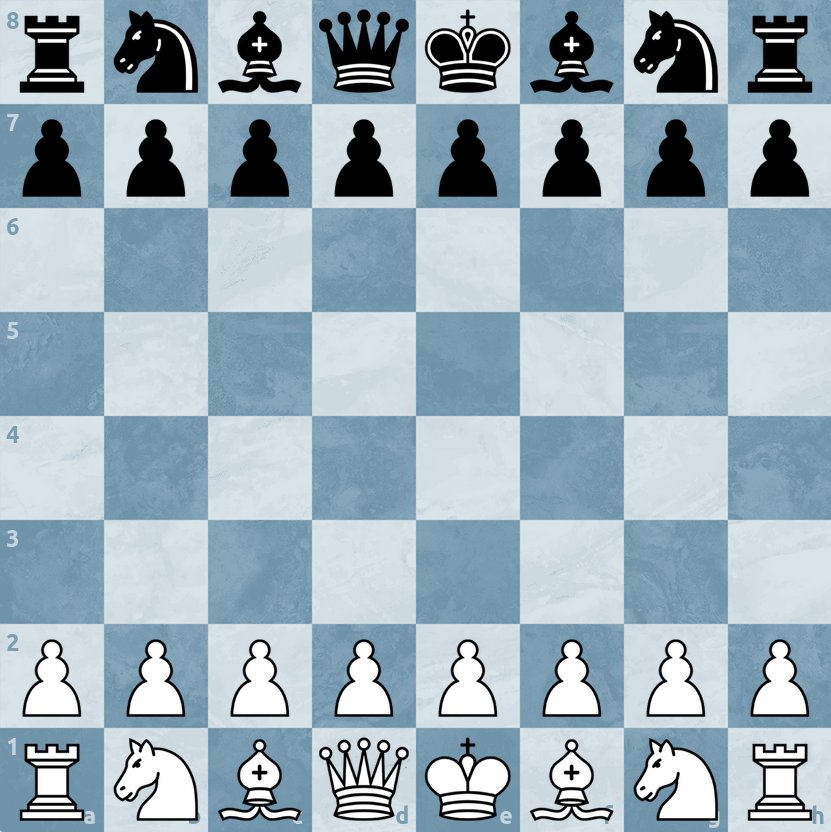
\includegraphics[width=0.6\textwidth]{jeuDepart.png}
    \vspace{0.5cm}
\end{minipage}

Le joueur avec les pièces blanches commence. Ensuite, chaque joueur joue à tour de rôle, un déplacement de pièce par tour.

\subsection{Déplacements des Pièces}
Les déplacements sont propres à chaque type de pièce :
\vspace{0.5cm}

\begin{itemize}
    \item \begin{minipage}{0.45\textwidth}
        \textbf{Déplacement du pion :} \\
        Le pion avance uniquement en ligne droite, d'une case à la fois. Toutefois, lors de son premier déplacement, 
        il a la possibilité d'avancer de deux cases. Contrairement à son déplacement habituel, le pion capture les pièces
         adverses en diagonale, en se déplaçant d'une case.
    \end{minipage}
    \hspace{0.05\textwidth}
    \begin{minipage}{0.45\textwidth}
        \centering
        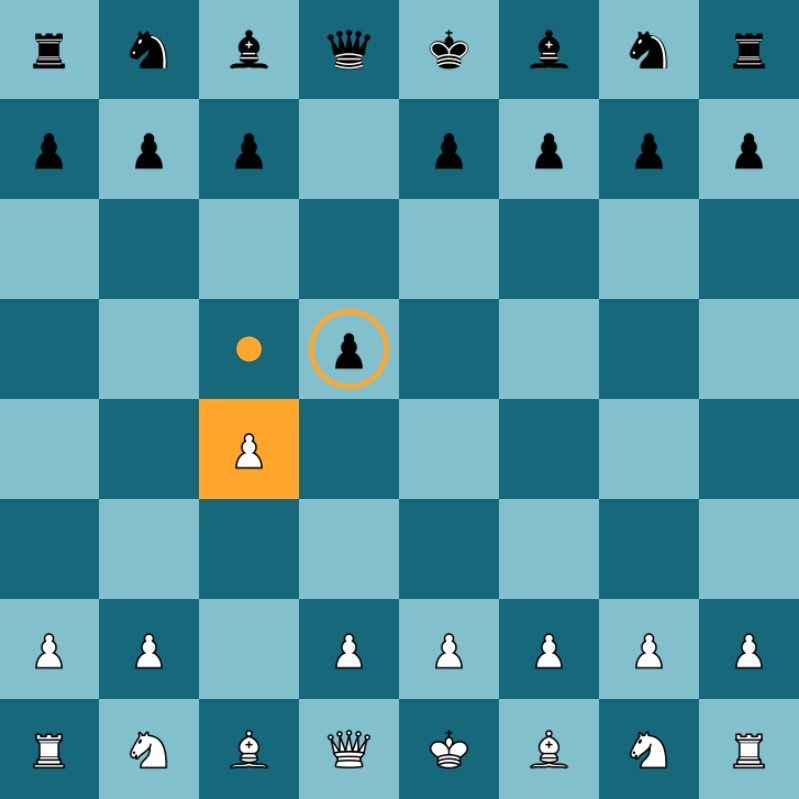
\includegraphics[width=\textwidth]{pionMove.png}
    \end{minipage}

    \vspace{0.5cm}

    \item \begin{minipage}{0.45\textwidth}
        \textbf{Déplacement du cavalier :} \\
        Le cavalier a un déplacement unique en forme de "L", ce qui signifie qu'il se déplace de deux cases dans une direction,
        puis d'une case perpendiculairement (ou inversement). C'est la seule pièce capable de sauter par-dessus d'autres 
        pièces sur l'échiquier.
    \end{minipage}
    \hspace{0.05\textwidth}
    \begin{minipage}{0.45\textwidth}
        \centering
        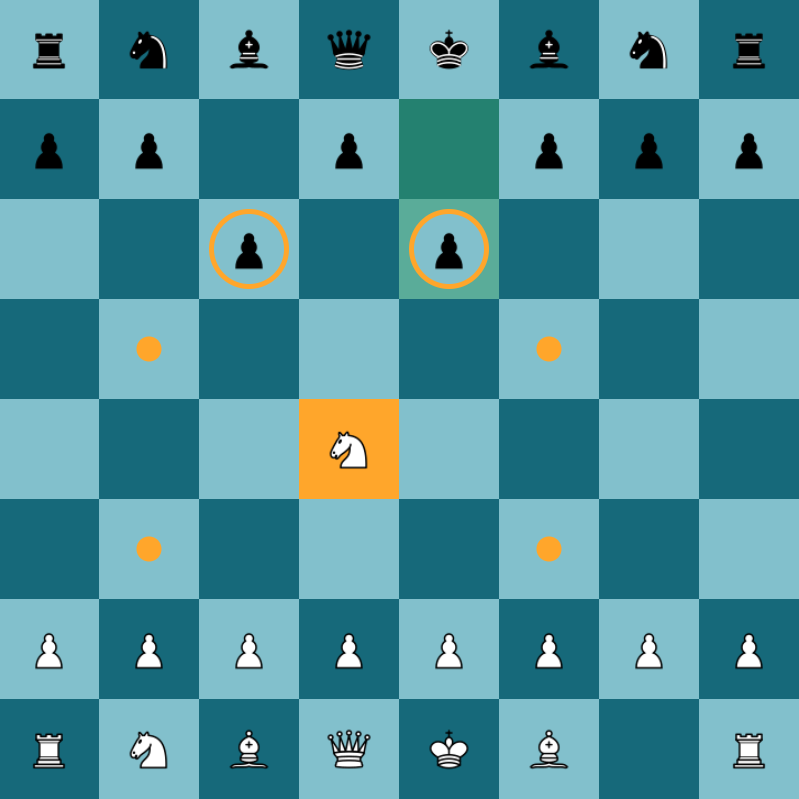
\includegraphics[width=\textwidth]{cavalierMove.png}
    \end{minipage}

    \vspace{0.5cm}

    \item \begin{minipage}{0.45\textwidth}
        \textbf{Déplacement du fou :} \\
        Le fou se déplace en diagonale sur un nombre illimité de cases, tant qu'il n'est pas bloqué par une autre pièce.
         Chaque fou reste toujours sur des cases de la couleur d'où il a commencé (blanches ou noires).
    \end{minipage}
    \hspace{0.05\textwidth}
    \begin{minipage}{0.45\textwidth}
        \centering
        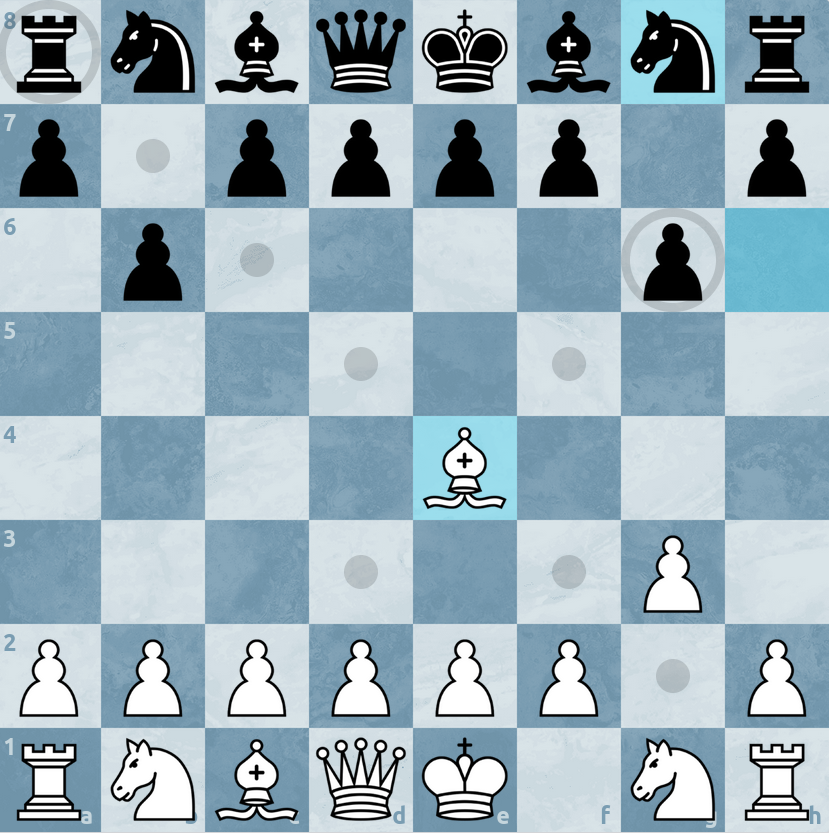
\includegraphics[width=\textwidth]{fouMove.png}
    \end{minipage}

    \vspace{0.5cm}

    \item \begin{minipage}{0.45\textwidth}
        \textbf{Déplacement de la tour :} \\
        La tour peut se déplacer de manière illimitée en ligne droite, que ce soit horizontalement ou verticalement.
        Sa puissance réside dans sa capacité à contrôler des colonnes et des rangées entières.
    \end{minipage}
    \hspace{0.05\textwidth}
    \begin{minipage}{0.45\textwidth}
        \centering
        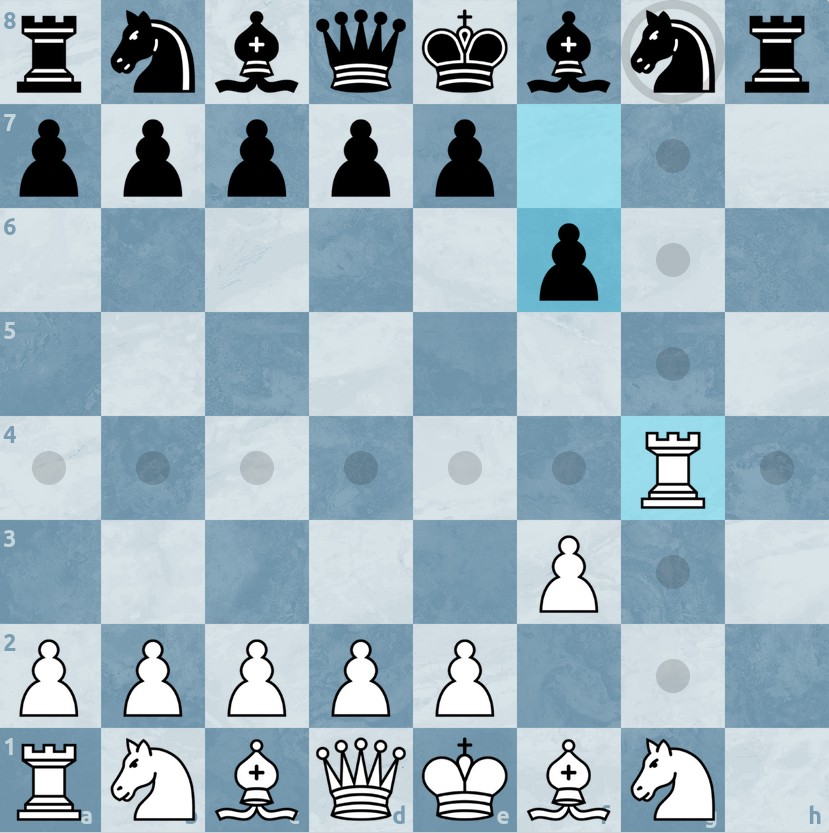
\includegraphics[width=\textwidth]{tourMove.png}
    \end{minipage}

    \vspace{0.5cm}

    \item \begin{minipage}{0.45\textwidth}
        \textbf{Déplacement de la dame :} \\
        La dame est la pièce la plus puissante du jeu. Elle combine les capacités de déplacement du fou et de la tour:
        elle peut se déplacer d'un nombre illimité de cases horizontalement, verticalement ou en diagonale.
    \end{minipage}
    \hspace{0.05\textwidth}
    \begin{minipage}{0.45\textwidth}
        \centering
        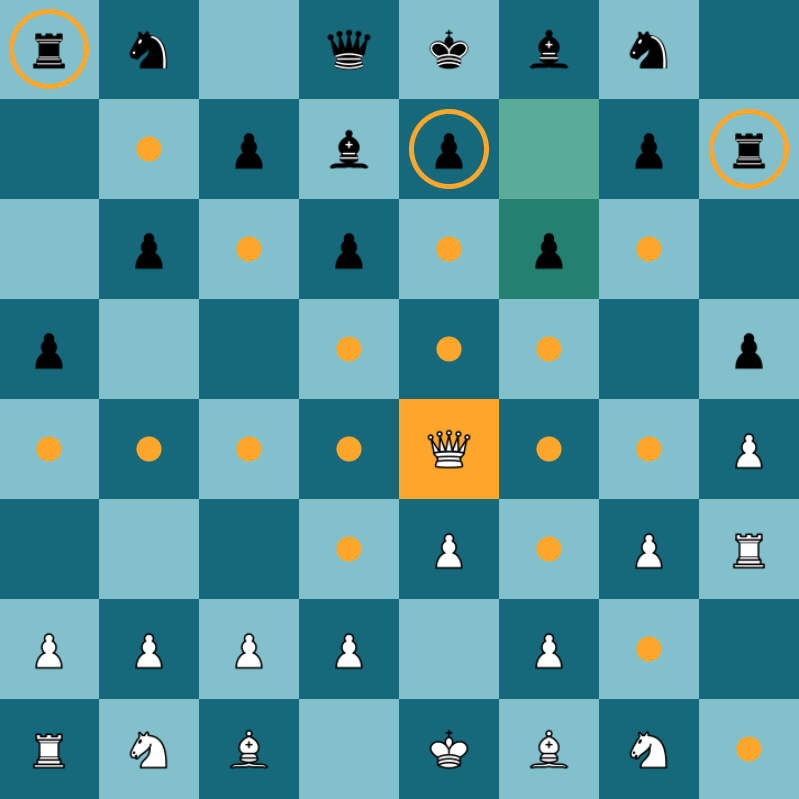
\includegraphics[width=\textwidth]{dameMove.png}
    \end{minipage}

    \vspace{0.5cm}

    \item \begin{minipage}{0.45\textwidth}
        \textbf{Déplacement du roi :} \\
        Le roi peut se déplacer d'une case dans n'importe quelle direction: horizontalement, verticalement ou en diagonale.
        Bien qu'il soit la pièce la plus importante, son mouvement limité le rend vulnérable.
    \end{minipage}
    \hspace{0.05\textwidth}
    \begin{minipage}{0.45\textwidth}
        \centering
        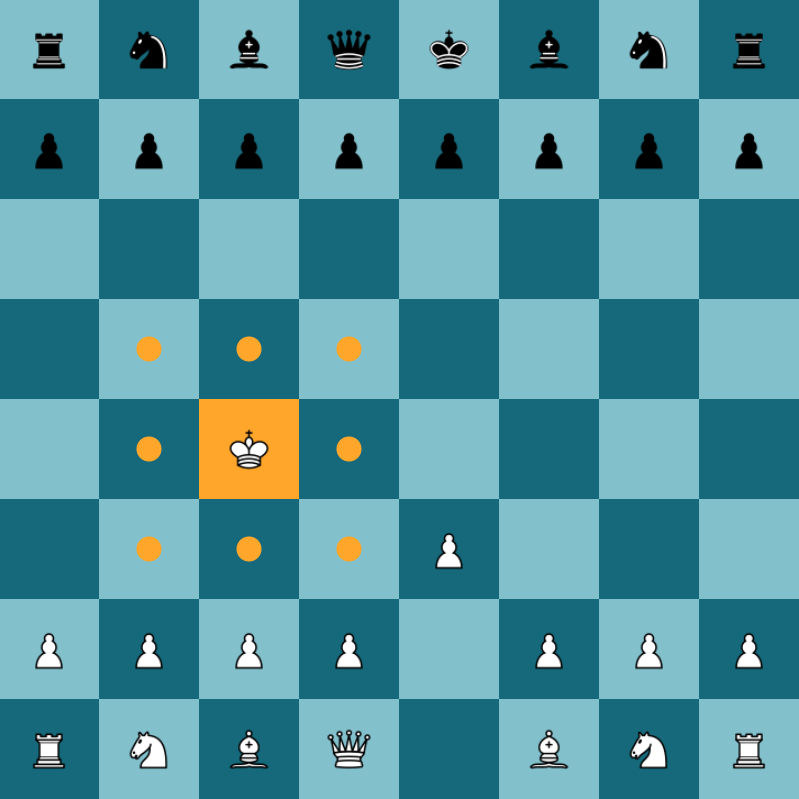
\includegraphics[width=\textwidth]{roiMove.png}
    \end{minipage}

\end{itemize}

\vspace{0.5cm}

Parfois, les déplacements peuvent être limités par des règles spécifiques comme le \textbf{clouage}. Voyons ces règles en détail.

\subsection{Règles Spécifiques}
\paragraph{-Clouage} Si une pièce défend une attaque au roi en se positionnant devant cette dernière, on dit qu'elle est \textbf{clouée}
 et ne peut pas bouger. En effet, il est interdit de mettre son roi en échec volontairement par l'une de ses propres actions.

 \noindent
 \begin{minipage}{0.48\textwidth}
     \centering
     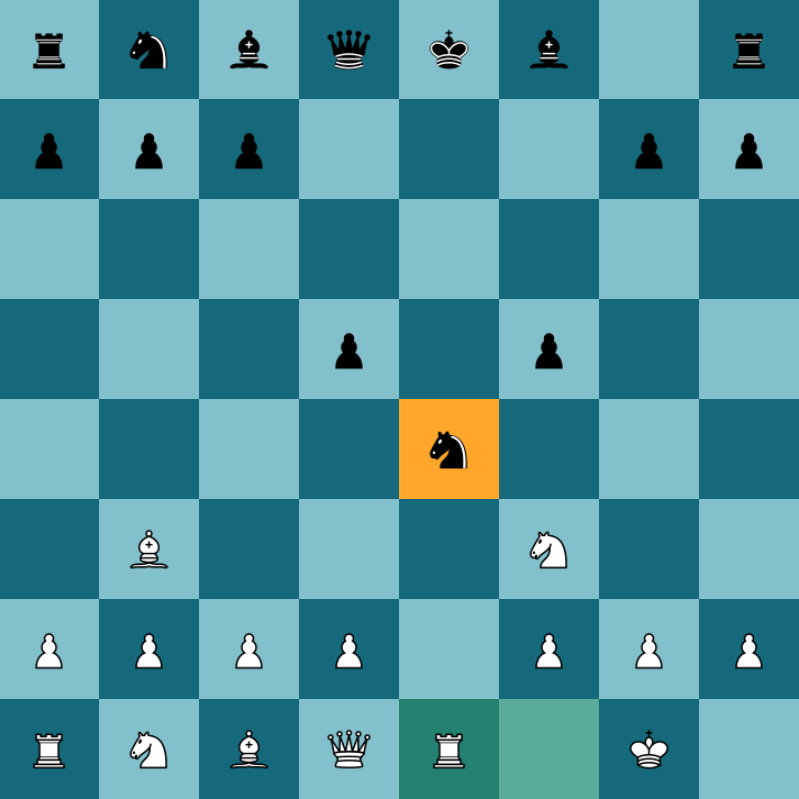
\includegraphics[width=\textwidth, height=\textwidth]{clouage1.png}
     \vspace{0.5cm}
    \textbf{Exemple de clouage}
 \end{minipage}
 \hfill
 \begin{minipage}{0.48\textwidth}
     \centering
     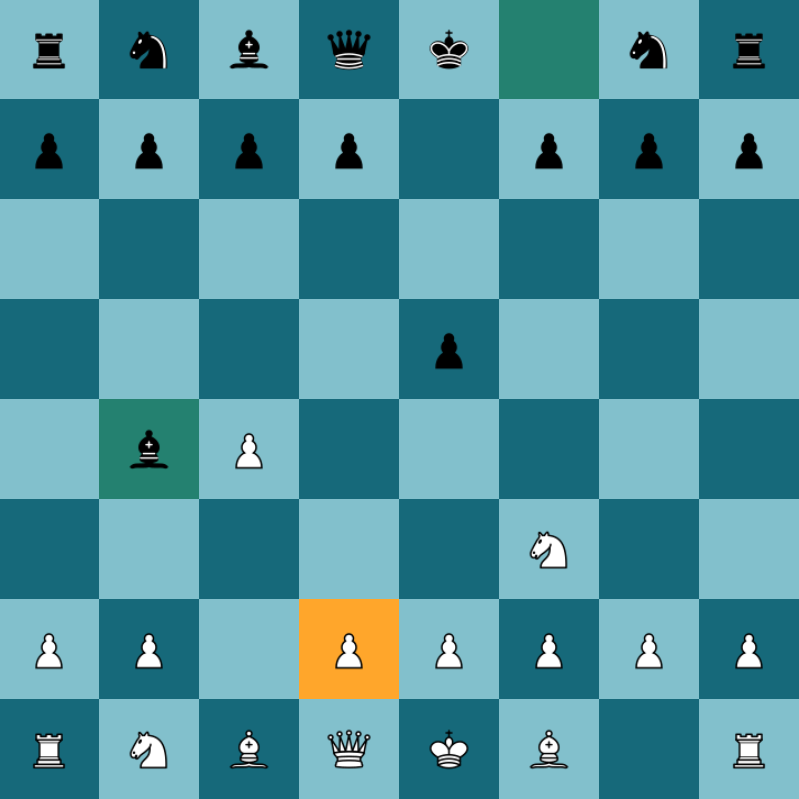
\includegraphics[width=\textwidth, height=\textwidth]{clouage2.png}
     \vspace{0.5cm}
 \end{minipage}

\paragraph{-Roque} Le \textbf{roque} est un mouvement spécial impliquant le roi et une des tours, sous certaines conditions :
\begin{itemize}
    \item Le roi et la tour concernés n'ont jamais bougé depuis le début de la partie.
    \item Le roi ne doit pas être en échec, et aucune des cases qu'il traverse ou sur laquelle il atterrit ne doit être attaquée.
    \item Il ne doit y avoir aucune pièce entre le roi et la tour.
\end{itemize}

\noindent
\begin{minipage}{0.48\textwidth}
    \centering
    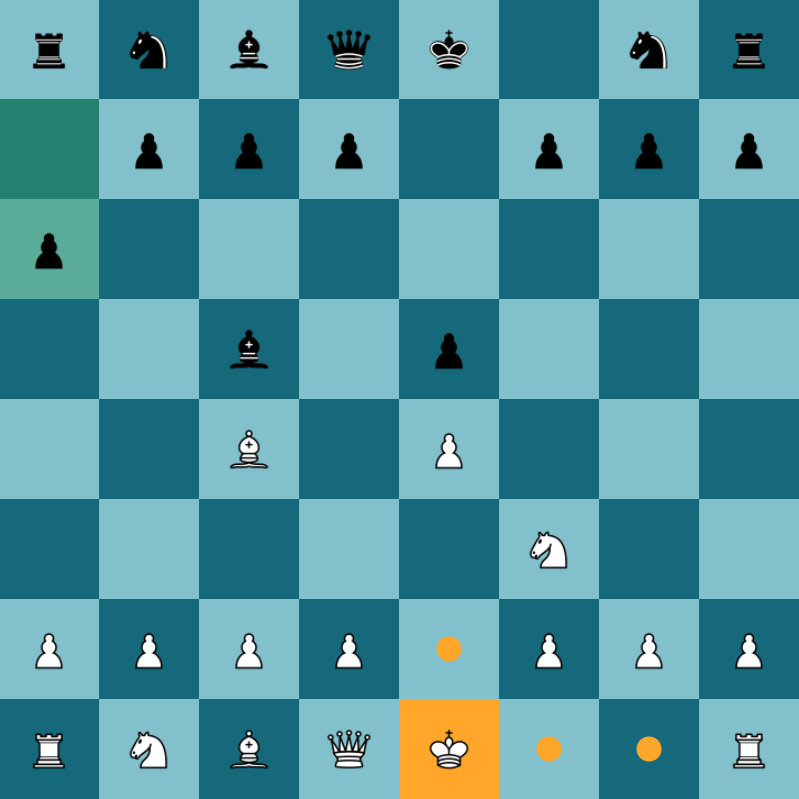
\includegraphics[width=\textwidth, height=\textwidth]{roque1.png}
    \vspace{0.5cm}
   \textbf{Exemple de roque}
\end{minipage}
\hfill
\begin{minipage}{0.48\textwidth}
    \centering
    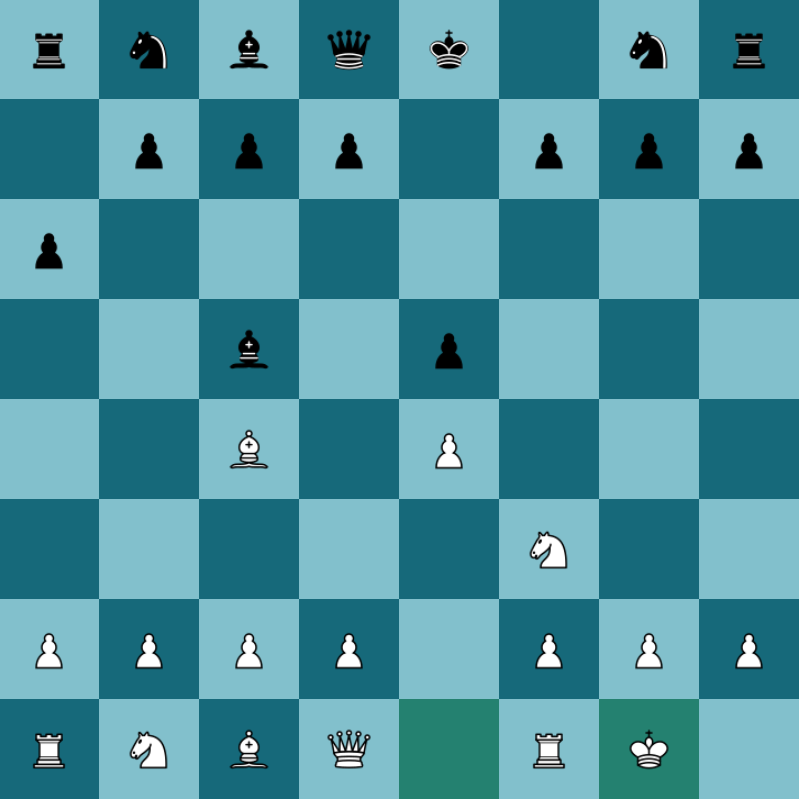
\includegraphics[width=\textwidth, height=\textwidth]{roque2.png}
    \vspace{0.5cm}
\end{minipage}

\paragraph{-Prise en Passant} Si un pion adverse avance de deux cases depuis sa position initiale et finit à côté d'un de nos pions,
 on peut le capturer \textbf{en passant}, mais uniquement au coup suivant.

 \noindent
 \begin{minipage}{0.48\textwidth}
     \centering
     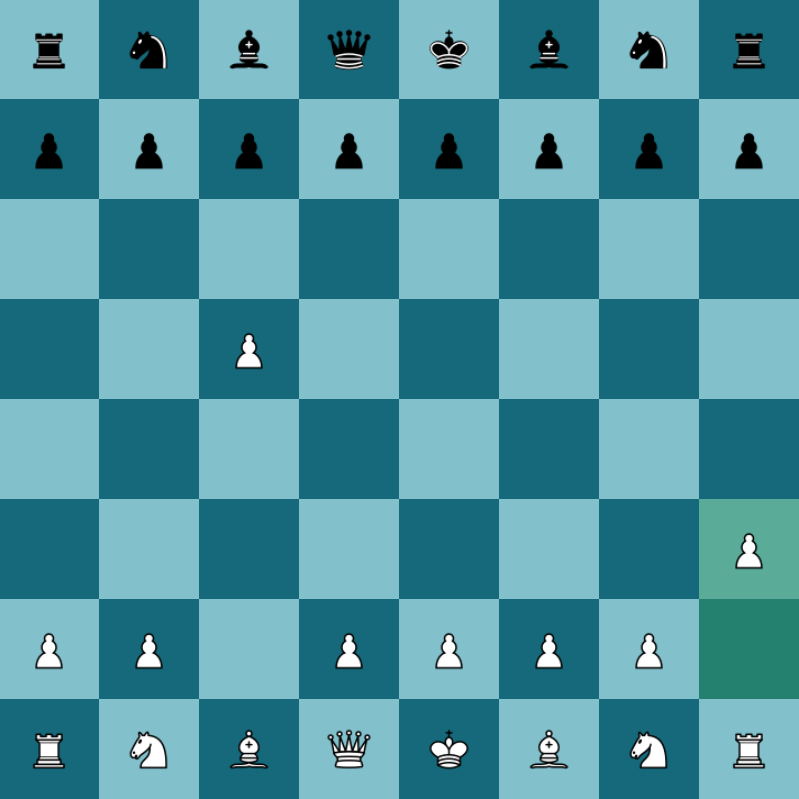
\includegraphics[width=\textwidth, height=\textwidth]{enpassant1.png}
     \vspace{0.5cm}
    \textbf{Exemple de en passant}
 \end{minipage}
 \hfill
 \begin{minipage}{0.48\textwidth}
     \centering
     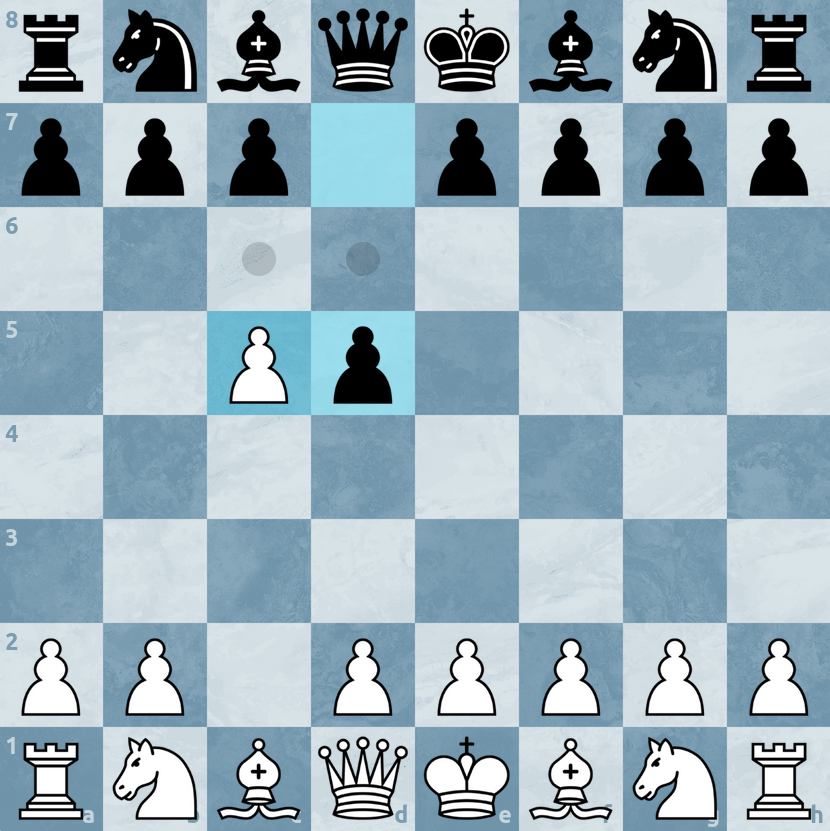
\includegraphics[width=\textwidth, height=\textwidth]{enpassant2.png}
     \vspace{0.5cm}
 \end{minipage}

\paragraph{-Promotion du Pion} Si un pion atteint la dernière rangée de l'échiquier, il peut être promu en dame,
 tour, fou ou cavalier. La promotion du pion est souvent synonyme d'avantage conséquent et peut mener à une victoire.

 \noindent
 \begin{minipage}{0.48\textwidth}
     \centering
     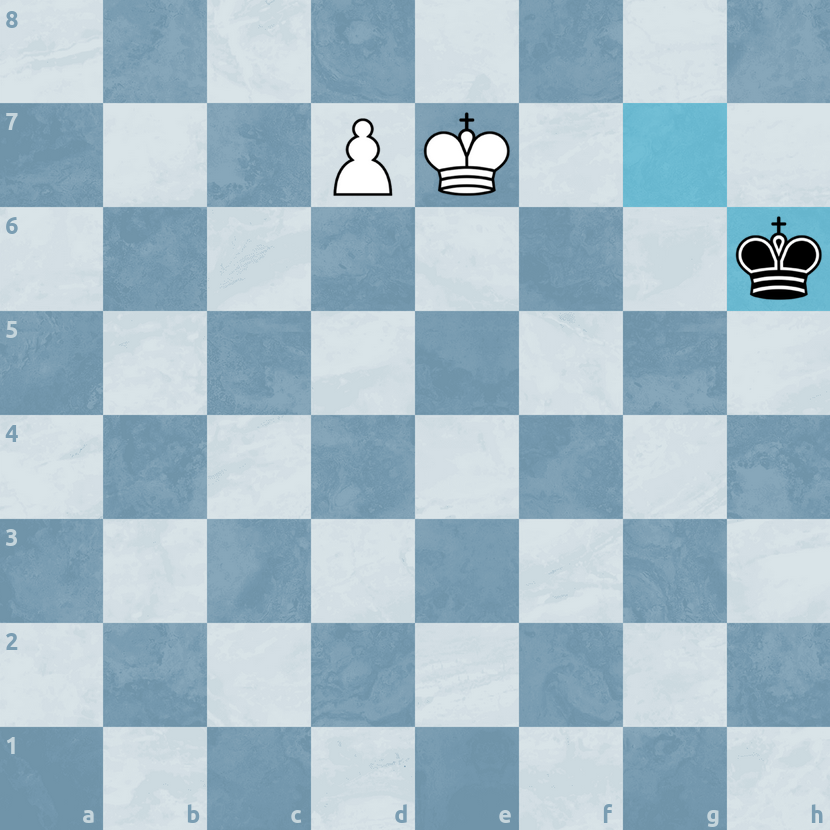
\includegraphics[width=\textwidth, height=\textwidth]{promotion1.png}
     \vspace{0.5cm}
    \textbf{Exemple de promotion}
 \end{minipage}
 \hfill
 \begin{minipage}{0.48\textwidth}
     \centering
     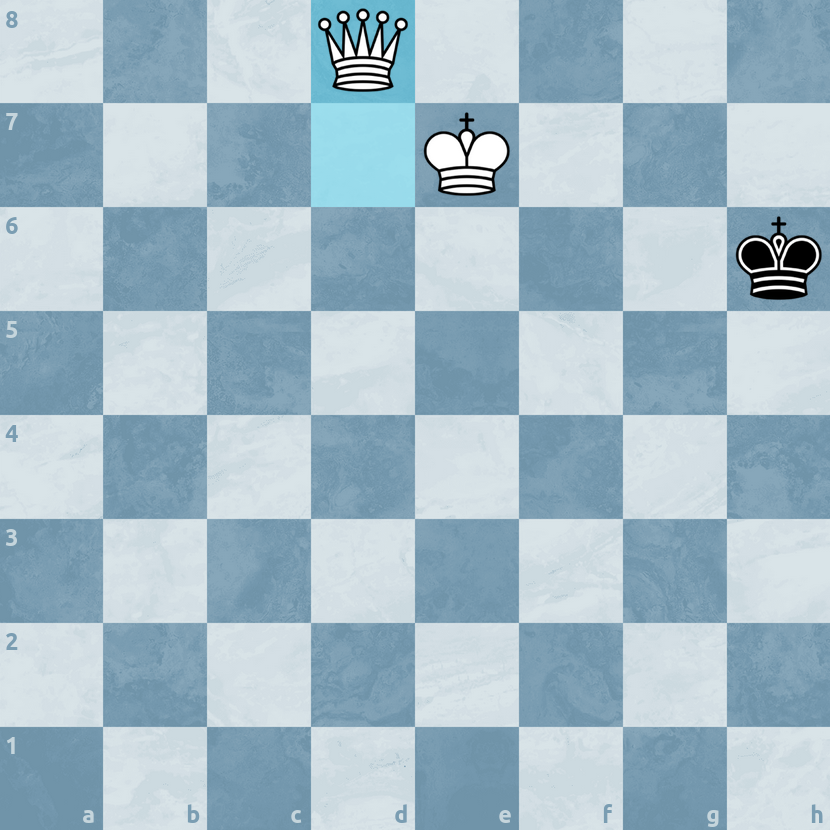
\includegraphics[width=\textwidth, height=\textwidth]{promotion2.png}
     \vspace{0.5cm}
 \end{minipage}

\subsection{Fin de Partie}
Une partie d'échecs peut se terminer de plusieurs façons :
\begin{itemize}
    \item \textbf{Échec et mat} : le roi est attaqué et aucun coup légal ne peut le sauver, ce qui donne la victoire à l'adversaire.
    \item \textbf{Pat} : un joueur n'a aucun coup légal à jouer et son roi n'est pas en échec, entraînant une nulle.
    \item \textbf{Manque de matériel} : si seuls les rois, ou un roi et un fou/cavalier, restent sur l'échiquier, un mat devient impossible, ce qui entraîne une nulle.
    \item \textbf{Répétition de position} : une même position exacte apparaît trois fois, entraînant une nulle.
    \item \textbf{Règle des 50 coups} : si aucun pion n'est déplacé ni pièce capturée pendant 50 coups consécutifs, la partie est déclarée nulle.
    \item \textbf{Abandon} : un joueur peut décider d'abandonner si sa position devient trop défavorable.
    \item \textbf{Accord mutuel} : les deux joueurs conviennent de déclarer une nulle lorsqu'aucun ne voit de progrès réaliste possible.
    \item \textbf{Dépassement de temps} : un joueur perd si son chronomètre s'écoule avant qu'il ne joue, sauf si l'adversaire n'a pas assez de matériel pour mater.
\end{itemize}



\section{Structures de données et Algorithmes}
\label{DataStruct}

\subsection{Plateau sous forme de bitmaps}
Un échiquier est finalement une matrice 8x8 (64 cases donc) sur lesquelles il y a une pièce, ou non. On voit ici une
notion de binaire. Pour une pièce: "Blanche ou Noire", "Présente ou Non" (pour les cases). Une méthode existe pour
représenter l'échiquier en se servant de bitmaps plutôt que d'utiliser des arrays, vecteurs ou listes en deux dimensions.
Il s'agit du bitboard. On observera un gain de performance en temps et un gain d'espace énormes pour la représentation
de l'échiquier (et des règles spécifiques).\\
Comme on vient de le voir, sur une case, soit il y a une pièce, soit il n'y en a pas.
Encodons le fait qu'une case soit occupée par 1 et le fait qu'une case soit vide (libre) par 0. Il y a 64 cases au total.
Donc, en attribuant un indice à chaque case (de 0 à 63), on va pouvoir chiffrer l'échiquier par un entier de 64 bits.
Chaque bit de cet entier est à 0 ou à 1. S'il est à 0 pour l'indice i, alors la case i est libre. S'il est à 1, alors la
case i est occupée. Un entier n'est cependant pas suffisant, car il faut pouvoir différencier les types de pièce, ainsi
que la couleur des pièces (noires ou blanches). Il y a au total 6 types de pièces aux échecs: le Pion, le Cavalier, le Fou,
la Tour, la Dame, le Roi. Donc finalement, on aura besoin de 12 entiers codés sur 64 bits, car 6 pour les types de pièces
blanches et 6 pour les types de pièces noires.
\\Il est important de noter que cela n'est pas réalisable pour des ordinateurs qui possèdent une architecture en 32 bits.
Aujourd'hui, la quasi-totalité des ordinateurs utilise du 64 bits, donc il ne faut pas trop s'en soucier. C'est néanmoins
crucial de relever les inconvénients des méthodes que l'on va utiliser pour ce projet. Un autre désavantage de cette méthode
est le fait qu'il faudra faire une gymnastique pour "décoder" pour l'humain une position. En effet, si l'on prend l'entier
112, on ne visualise pas (du tout) la position, même si l'ordinateur si.
Retenons aussi que l'on aura à faire à des représentations et opérations binaires, pour lesquelles un ordinateur est très
performant. En Java, chaque entier sera un long (type primitif).
\\Il faut aussi se pencher sur les règles spécifiques que l'on encodera avec les 12 bitmaps pour représenter une position
dans son entièreté. Effectivement, pour le moment, nous n'avons que l'emplacement des pièces sur l'échiquier. Mais une position
est aussi décrite par ses règles, c'est un état de jeu. Les règles à prendre en compte sont:\\
\begin{itemize}
    \item En passant: Il faut utiliser 1 bit comme flag, 1 si en passant possible et 0 sinon. Il y a au total 16 cases cibles où
    un en passant peut se produire. On utilise donc 4 bits (16 valeurs) supplémentaires. Au total donc, 5 bits.
    \item Roques: on compte le grand roque et le petit roque des deux côtés (noirs et blancs). On a donc besoin de 4 bits.
    \item Temps à la pendule: Pour les blancs et les noirs, on doit savoir combien de temps il reste à chaque état du jeu. Si
    l'on se dit que chaque joueur dispose de 24h pour une partie en prenant large, il faut coder 86 400 000 (en ms). Pour cela,
    on a besoin de 27 bits. Mais il s'agit de 27 bits de chaque côté car il y a les blancs et les noirs. Donc au total, 54 bits ici.
    \item Règle des 50 coups: Pour le nombre de coups sans capture ou mouvement de pion, on se sert de 6 bits (entre 0 et 50).
    \item Nombre de "FullMoves": Pour se souvenir du nombre de coups total de la partie, on va prendre large et utiliser 10 bits,
    ce qui nous donne la possibilité d'avoir 1000 coups.\\
\end{itemize}

Si l'on effectue le total, une position est codée sur 12*64 + 5 + 4 + 54 + 6 + 10 = 847 bits.
C'est un gain très conséquent qui va notamment nous permettre par exemple de chercher à une profondeur plus grande pour la partie
Intelligence Artificielle. Il y a quelques détails en ce qui concerne les performances dans les parties \ref{DataStruct} Structures de données et
\ref{AI} Intelligence Artificielle dans le rapport notamment.

\subsection{Historique des coups}
\par La liste (doublement) chaînée a été choisie par le groupe afin de stocker les coups qui représentent l'historique de jeu.
En effet, l'insertion et la suppression sont des opérations réalisables en O(1). L'historique est alors plus flexible et les
modifications sur l'historique sont assez efficaces. Pour revenir à un certain coup de la partie, qu'il s'agisse d'un undo ou redo,
nous sommes en O(n), n étant le nombre de coups. En revanche, il y a certains cas où cette approche n'est pas très optimale.
Par exemple, pour les parties (très) longues. En effet, la surcharge en mémoire (due aux références) et le coût en temps pour
parcourir la liste peuvent devenir problématiques. Notons néanmoins que c'est un problème pour quasiment toutes les structures de
données pour ce cas-là. Grâce au chaînage, se promener dans l'historique devient très pratique et plutôt performant.
Cependant, cette solution comporte l'inconvénient d'une complexité plus élevée en termes de maintenance et de gestion de la mémoire.
\'A titre d'exemple, trois classes différentes dans le code ont dues être créées afin d'implémenter cette solution avec liste doublement chaînée.
En bref, chaque noeud (ou élément) de la liste est représenté par une configuration de la partie, soit un GameState.
Ces noeuds sont reliés entre eux par des coups, permettant de jouer ou annuler un coup afin de traverser les états de jeu
de la partie.\\
Voici à quoi ressemble l'historique des coups d'une partie dans notre jeu en GUI:\\

\begin{figure}[h]
    \caption{Exemple historique de coups}
    \centering
    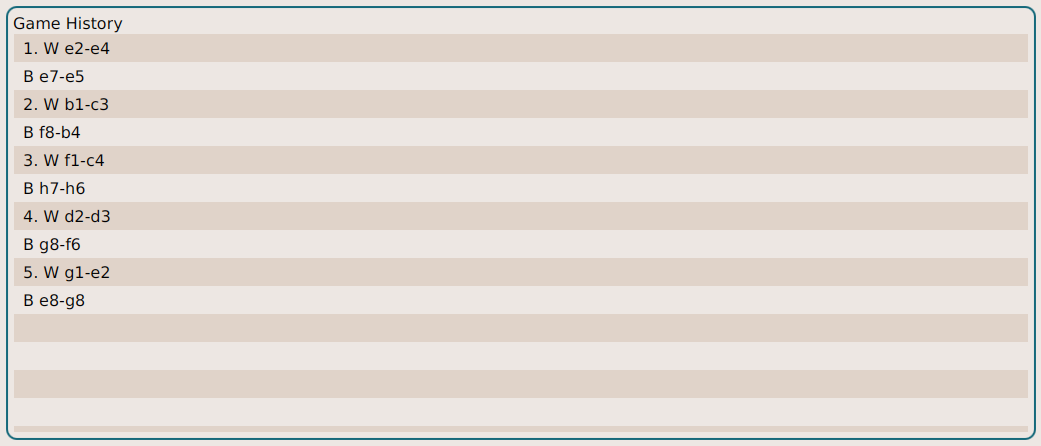
\includegraphics[width=\textwidth,height=5.0cm,keepaspectratio]{historique-coups}
\end{figure}

\subsection{Intelligence Artificielle} \label{AI}
\subsubsection{Heuristiques}
Afin de coder une bonne heuristique, aux échecs, il faut prendre en compte beaucoup d'éléments et revenir aux bases du jeu.
Notamment, il faut savoir ce qui importe dans une position, ce qui donne l'avantage ou ce qui assure une égalité. Essentiellement,
on se contente de vérifier certains points clés qui vont nous permettre d'émettre une évaluation sur une position.
Rappelons que le facteur de branchement aux échecs approche les 35.\\
Il y a de nombreux éléments à prendre en compte, et en voici certainement les plus impactants:
\begin{itemize}
    \item Le Matériel: chaque pièce (sauf peut-être le roi) possède une valeur. On va donc s'occuper de compter pour les 2 camps le "potentiel"
    dans une position. Plus on a de matériel (pièces donc), plus on a de chances d'avoir l'avantage, en particulier par un bon contrôle de l'échiquier.
    \item La sécurité du Roi: Le Roi est la pièce la plus importante aux échecs, et souvent, le joueur qui a un avantage est celui qui va
    avoir un Roi qui n'est pas en danger. Pour estimer cela, on peut en particulier vérifier le nombre de coups où l'on peut mettre le Roi en échec,
    combien de coups permettent de l'en sortir, et la fréquence des échecs. Plus un Roi est vulnérable, plus il y aura des possibilités
    de le mettre en échec.
    \item Le contrôle du centre: Aux échecs, le centre est un emplacement clé, puisqu'il peut donner un accès efficace à toutes les parties de
    l'échiquier. Généralement, obtenir un bon contrôle du centre est un facteur qui va jouer dans l'évaluation d'une position.
    \item L'activité: Si l'on a peu de coups légaux que l'on peut jouer, c'est très souvent parce que l'on est en position de désavantage. Cela peut
    signifier que l'on est forcé à jouer certains coups.
    \item La structure de pions: Plus on aura une structure de pions solide, plus on aura de potentiel d'attaque et de défense puisque les pions sont
    des pièces "faibles" lorsqu'ils sont seuls et/ou non défendus.
    \item La promotion: Plus on a de pions avancés, plus on a de chance d'atteindre la dernière rangée et changer notre pion en une pièce plus importante,
    comme la Dame par exemple, nous donnant plus d'options.\\
\end{itemize}

Seulement ceux-là sont cités ici, mais en réalité, il y a plus de 20 points clés nous permettant d'évaluer une position de manière efficace.
Enfin, afin d'obtenir une bonne heuristique aux échecs, il faut considérer tous ces points et faire une somme. C'est la marche à suivre puisque
il s'agit d'un jeu à somme nulle, c'est-à-dire que le gain d'un joueur correspond exactement à la perte de l'autre. En d'autres termes, si un joueur gagne (+1), l'autre perd (-1), et si la partie est nulle, aucun des deux joueurs ne gagne ni ne perd (0-0). \\
Dans ce projet, le groupe a développé une multitude d'heuristiques permettant d'évaluer des positions. Essentiellement, elles peuvent être regroupées
en deux catégories: Heuristiques "STANDARD" et Heuristiques "ENDGAME" ("Fin de partie"). En se servant du design pattern Composite, on combine les
heuristiques codées afin de se baser sur "beaucoup" de facteurs dans le but d'obtenir une évaluation d'une position la plus précise possible. Ainsi,
l'Intelligence Artificielle (MiniMax et AlphaBeta) utilise ces évaluations pour en déduire un "meilleur coup". STANDARD et ENDGAME sont les 
heuristiques par défaut lorsque l'IA est lancée. Le programme vérifie à tout moment (après chaque coup joué ou après chaque coup repris)
si le jeu se trouve être dans un stade de fin de partie ou non. Si la configuration est considérée être une fin de partie, alors l'heuristique utilisée
parl'IA devient ENDGAME, afin de prendre en compte des facteurs propres aux fins de partie. Autrement, elle utilise la STANDARD.\\
Voici quelques exemples d'heuristiques que le groupe a pu développer:
\begin{itemize}
    \item KingSafetyHeuristic : Une heuristique évaluant la sécurité du Roi.
    \item MaterialHeuristic : Une heuristique évaluant le matériel disponible de chaque côté.
    \item SpaceControlHeuristic : Une heuristique évaluant le contrôle de l'échiquier en se basant notamment sur le nombre
    de coups possibles.
    \item DevelopmentHeuristic : Une heuristique évaluant le développement des pièces sur l'échiquier.
    \item KingActivityHeuristic : Une heuristique évaluant l'activité du Roi (utilisée pour les fins de partie).
\end{itemize}

\subsubsection{Algorithmes}
Dans cette partie Intelligence Artificielle, on va essentiellement se servir des 3 algorithmes suivants (dont 2 vus au dernier semestre):
\begin{itemize}
    \item MiniMax: Visant à retourner l'option la plus adéquate dans une certaine position, on utilise des arbres pour savoir quelle branche va être la
    plus intéressante, que ce soit pour l'ami, comme pour l'ennemi. On est en O($b^d$) en temps, où b est le facteur de branchement et d la profondeur.
    En espace, c'est du O(d), soit le nombre de niveaux dans l'arbre pour une approche basée sur du DFS.
    \item AlphaBeta-pruning: Cet algorithme se repose sur MiniMax, mais peut permettre d'aller à une profondeur deux fois plus grande si les nœuds de
    l'arbre sont organisés du plus petit au plus grand. Ici, la valeur des nœuds va être une évaluation. La complexité en espace ne change pas, mais
    en temps nous sommes donc en O($b^p$) où p = d/2.
    \item MonteCarloTreeSearch:
    Celui-ci peut se décomposer en quatre étapes : \textbf{Selection}, \textbf{Expansion}, \textbf{Simulation}, et \textbf{BackPropagation}. Pour faire simple, on va choisir (Selection) des branches à explorer. Cela peut être les nœuds qui vont être impactants sur la recherche du meilleur coup, ou encore des nœuds qui n'ont pas encore été explorés. Il s'agit de l'UCT (Upper Confidence bound applied to Trees).\
    L'UCT est une formule permettant d'équilibrer l'exploration et l'exploitation dans la sélection des coups :
    \begin{equation}
    UCT = \frac{w(i)}{s(i)} + C \sqrt{\frac{\ln(N)}{s(i)}}
    \end{equation}
    où :
    \begin{itemize}
        \item $w(i)$ est le nombre de victoires du nœud $i$.
        \item $s(i)$ est le nombre total de simulations passées par ce nœud.
        \item $N$ est le nombre total de simulations effectuées depuis la racine de l'arbre.
        \item $C$ est un coefficient ajustable permettant de pondérer l'exploration.\
    \end{itemize} 

    L’UCT permet ainsi d’équilibrer l’exploration de nouveaux coups et l’exploitation des meilleurs coups déjà identifiés.
    Cela permet à l’algorithme MCTS de converger vers des coups optimaux tout en continuant à explorer de nouvelles options lorsque cela est nécessaire.
    Ensuite, après avoir choisi la branche, on se positionne à la feuille de cette branche,
    puis on simule un coup aléatoirement (Expansion) et on l'évalue. Maintenant, à partir de ce nouveau nœud, on simule une partie ou une pseudo-partie
    aléatoirement pour estimer le résultat potentiel. Finalement, lorsque l'on obtient un résultat, on fait remonter l'évaluation (BackPropagation)
    et/ou les informations importantes vers le haut de l'arbre pour plus tard agir en conséquence. En temps, on se rapproche de O(n*d), où n est le
    nombre de simulations effectuées, et d la profondeur moyenne. En espace, dans le pire des cas, on peut se trouver en O(N) où N est le nombre
    de simulations jouées. Maintenant, dans le cas moyen, on est en O($b^p$) avec d la profondeur et b le facteur de branchement.
    Cependant, dans le cadre de ce projet, MCTS n'est pas borné par une profondeur. On peut donc dire que l'on se trouve en O(N).\\
    En ce qui concerne la partie structures de données, le MCTS se base une classe Java, appelée dans le code 'TreeNodeMonteCarlo'.
    Comme son nom l'indique, il s'agit d'un objet représentant un noeud de l'arbre sur lequel l'algorithme va se dérouler.
    Essentiellement, cet objet va contenir les informations suivantes:
    \begin{itemize}
        \item GameState représentant la configuration de la partie
        \item Noeud parent (objet de même type)
        \item Noeuds enfants (objets de même type)
        \item Le nombre de victoires constatées depuis ce noeud
        \item Le nombre de visites de ce noeud (pour l'UCT et le winrate d'un coup)
        \item Le coup qui a amené à ce noeud depuis une configuration précédente
    \end{itemize}
    En reliant ces noeuds par des coups, on arrive à contruire un (pseudo-)arbre et à appliquer l'algorithme du Monte Carlo Tree Search dessus.
\end{itemize}

\par Notons que tous les algorithmes s'effectuent sur des arbres, et AlphaBeta ainsi que MiniMax se servent d'une heuristique pour évaluer chaque position.
PARLER DES OPTIMISATIONS D'IA MISES EN PLACES ET PEUT-ETRE CELLES ENVISAGÉES OU POSSIBLES;

\subsection{Zobrist hashing} \label{Zobrist}
Le Zobrist hashing est une fonction utilisée en particulier dans les jeux comme les échecs ou le Go, où le but est d'attribuer un codage "complexe" à
une position, pour éviter d'analyser une position plus d'une fois. Ainsi, on peut gagner en performance, notamment dans les algorithmes d'IA, où les
états de jeu peuvent se répéter un grand nombre de fois. On va se servir de ce qu'on appelle des "tables de transposition", qui sont des tables de
hachage indexées par une position. Dans notre cas, les positions sont encodées par 12 bitmaps, et quelques bits
supplémentaires pour les règles spécifiques. Pour chaque combinaison case-pièce, on va générer un nombre aléatoire. De cette façon, toutes les configurations
de plateaux vont être rencontrées. Le hachage va consister à combiner toutes ces chaînes de bits pour chaque configuration avec l'opérateur XOR,
pour à la fin obtenir un hachage final pour chaque position. Ainsi, en utilisant une HashMap, on va conserver tous les hachages représantant toutes les
configurations possibles pour les utiliser plus tard. Par exemple, pour la règle "Threefold repetition", il faut vérifier si dans cette table de hachage
il existe un hachage H tel que H $\ge$ 3. Si c'est le cas, alors la partie se termine en égalité.
\\Donc, dans notre cas, on aura quelque chose de la sorte:\\
\begin{itemize}
    \item ZobristBoardTable[64][12]
    \item ZobristEnPassantTable[64]
    \item ZobristCastlingRightsTable[16]
    \item ZobristFiftyMoveRuleTable[51]
    \item ZobristFullMoveTable[1025]
\end{itemize}

\par Chaque élément sera donc en premier aléatoire, puis bits à bits, des opérations avec XOR seront réalisées. C'est avantageux car lorsque l'on joue
un coup, donc que l'on change l'état du jeu, il n'y a pas à tout recalculer. D'abord, on XOR le nombre aléatoire correspondant à la pièce qui quitte
sa case de départ, puis celui pour la case d'arrivée de cette pièce, et éventuellement changer les bits pour les règles spécifiques.
Pour l'IA, cette méthode sera clé car elle fera gagner en performance, car les états de jeu peuvent se répéter un grand nombre de fois (même si pas
toujours dans le même ordre).

\subsection{Cache}
Afin que le programme soit plus performant, le groupe a mis en place un système de "cache". COMPLETER.

\subsection{Bidirectional Map}
COMPLETER.

\subsection{Iterative Deepening}
COMPLETER.

\subsection{Code propre}
COMPLETER.


\section{Architecture du projet}
Nous avons décidé de présenter le projet sous une forme d'architecture MVC personnalisée. Cette architecture est particulièrement pratique pour nous, développeurs, aussi bien en termes de maintenance que d'extensibilité.

Les différents modules principaux de notre projet sont les suivants : \textbf{Model}, \textbf{Controller}, \textbf{Vue}, \textbf{Events}, \textbf{Utils}
et \textbf{Exceptions}. 

Voici l'architecture UML du projet : 

\begin{center}
    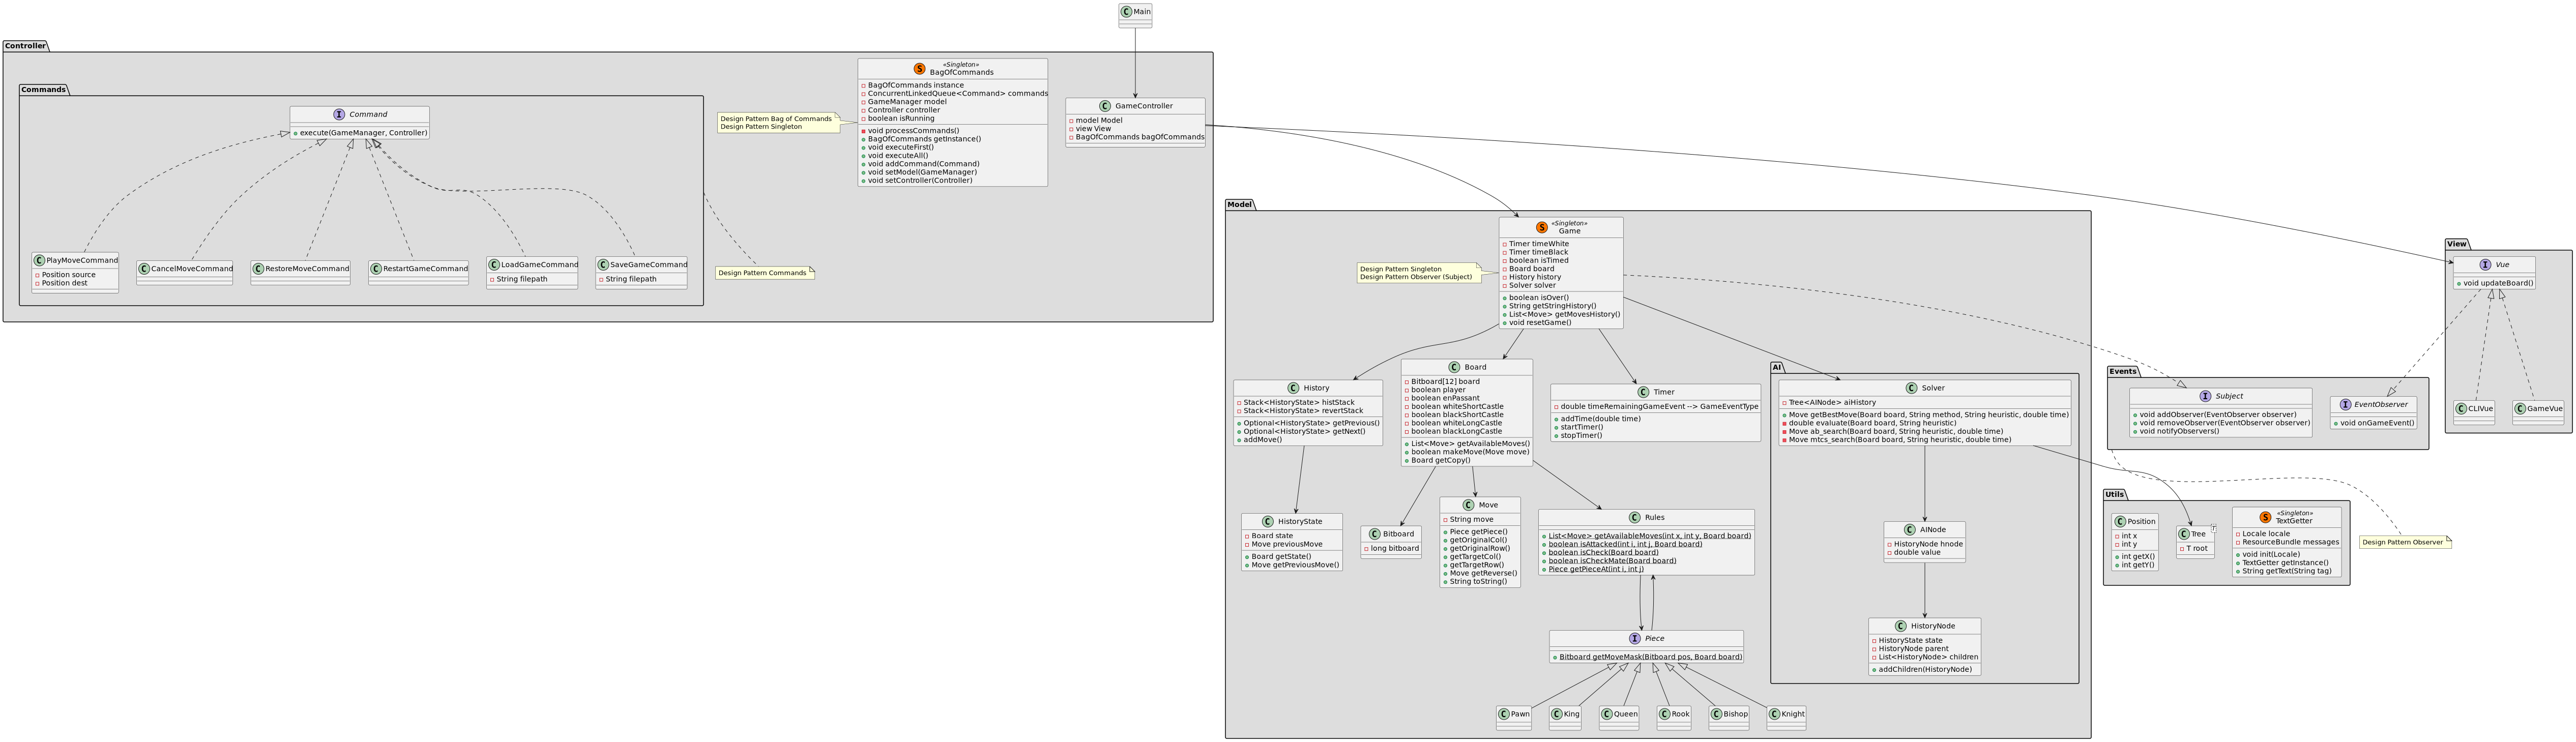
\includegraphics[width=\textwidth,height=\textheight,keepaspectratio]{archiUML}
\end{center}


\subsubsection{Description des Modules}

\begin{itemize}
    \item \textbf{Model} : Gère la logique métier du jeu, incluant l'état de la partie, les règles d'échecs et les fonctionnalités comme l'historique et le timer, et même l'Intelligence Artificielle.
    \item \textbf{Controller} : Sert d'intermédiaire entre la Vue et le Model. Il gère les événements utilisateurs et orchestre les interactions entre les différentes couches.
    \item \textbf{Vue} : Responsable de l'affichage et des interactions avec l'utilisateur, qu'il s'agisse d'une interface CLI ou graphique.
    \item \textbf{Events} : Implémente un système d'observateurs pour gérer les notifications et la communication asynchrone entre les modules.
    \item \textbf{Utils} : Contient des outils génériques comme le gestionnaire de textes internationalisés (\texttt{TextGetter}) et les algorithmes d'intelligence artificielle pour le jeu.
    \item \textbf{Exceptions} : Contient les types d'exceptions personnalisées qui peuvent survenir dans le programme et nous permettant d'agir en conséquence.
\end{itemize}

\subsubsection{Design Patterns Utilisés}

Les différents design patterns utilisés dans ce projet sont les suivants : 
\begin{itemize}
    \item \textbf{Singleton} : Utilisé pour la classe \texttt{Game} pour s'assurer qu'une seule instance de la partie est présente.
    La classe \texttt{BagOfCommands} utilise ce design pattern afin que la gestion des commandes ne soit gérée que par un seul bag.
    \item \textbf{MVC} : L'architecture principale du projet, séparant clairement la logique métier, l'affichage et la gestion des événements. C'est un MVC modifié,
 grâce au design pattern Observer qui va permettre d'envoyer des messages du Model vers la Vue. Cela permet notamment une meilleur flexibilité dans la
 gestion d'évènements.
    \item \textbf{Observer} : Permet de notifier la Vue des modifications dans le Model.
    \item \textbf{Command} : Utilisé pour simplifier le Controller. Chaque commande a un objectif précis, effectuer un certain traitement dans le Model.
    \item \textbf{Bag of Commands} : Utilisé pour gérer les Commandes. Nous pourrons gérer l'ajout de plusieurs commandes en parallèle.
    \item \textbf{Composite} : Utilisé pour combiner les heuristiques qui sont manipulées par l'Intelligence Artificielle.
\end{itemize}


\section{Performances et Limitations}
\subsection{Traces}
PRINT TRACES.

\subsection{Optimisations Intelligence Artificielle}
COMPARAISON ALPHA\_BETA, ALPHA\_BETA\_PARALLEL, ALPHA\_BETA\_IT

\subsection{Profondeur de recherche}
d = 6+ très long.

\subsection{Vue}
JavaFX, bien que pratique pour développer des GUI en Java, présente des limites en termes de performance, en particulier en ce qui concerne
la fluidité et les animations. En effectuant quelques recherches, on se rend compte que l'engine de rendu du framework repose principalement
sur Java2D et utilise une pipeline GPU limitée, ce qui peut causer des ralentissements, surtout pour les logiciels nécessitant du refresh
fréquent. Java est globalement un langage rapide, mais il est limité. Si le projet avait été développé en C++, avec notamment
l'aide d'OpenGL, la vue serait bien plus efficace. Sinon, en comparaison, l'utilisation d'un engine dédié comme Unity ou Godot permettrait
un meilleur rendu général, tandis qu'une approche basée sur les technologies web (HTML, CSS, WebGL) offrirait une
optimisation native des performances. Finalement, JavaFx se trouve être une solution pour l'interface graphique dans notre cas, et même si
pratique et bien architecturé, reste limité en termes de performances graphiques.

\section{Critiques et Perspectives}
Ce projet a été décomposé en une soixantaine de besoins afin d'être réalisé. Même si cette réalisation a été plutôt atteignaible, il est important de
faire part des points faibles de l'application, de ses points forts, et potentiellement des nouvelles fonctionnalités ou améliorations qui pourraient ou 
auraient pu voir le jour dans le cadre de cette U.E.
\subsection{Critiques Négatives}
\subsubsection{MonteCarloTreeSearch}
Le Monte Carlo Tree Search (MCTS) est largement utilisé dans les jeux de stratégie tels que le Go, où la non-présence d'heuristiques efficaces rend les méthodes classiques d'IA comme AlphaBeta moins adaptées. Cependant, aux échecs, MCTS est rarement employé à cause d'une multitude de limitations.
Premièrement, les échecs bénéficient d'évaluations positionnelles efficaces et d'une base théorique bien établie, ce qui permet aux algorithmes classiques comme Minimax avec AlphaBeta d'explorer l'arbre de jeu de manière plus efficace. Contrairement à des derniers, MCTS ne se base pas sur des critères d'évaluation et d'optimisations. Ensuite, MCTS est intrinsèquement plus lent que les méthodes basées sur Minimax. En effet, sans optimisation spécifique, il doit effectuer un grand nombre de simulations pour obtenir une estimation intéressante de la valeur d'un GameState. Dans un jeu comme les échecs, où le facteur de branchement moyen est élevé, MCTS a besoin d'un (très) grand nombre d'itérations pour converger vers des décisions "optimales" comparables à celles d'Alpha-Beta Pruning. La simulation de coups est très "Brute-Force", surtout sans optimisation, car le choix des coups par l'algorithme s'effectue de manière complètement aléatoire (pour la partie simulations).
Enfin, les engines d'échecs modernes tirent parti d'optimisations telles que le move ordering, des bibliothèques d'ouvertures, améliorant ainsi les performances d'Alpha-Beta Pruning. Bien que le MCTS puisse être optimisé par des techniques spécifiques d'IA comme les réseaux de neuronnes, son efficacité brute sans ces améliorations reste inférieure aux méthodes classiques pour les échecs. Maintenant, le groupe admet que son implémentation du MCTS est 
lente de base, notamment à cause d'un grand nombre de deep copies d'objets GameState
Ainsi, bien que MCTS soit une approche puissante pour certains jeux, son application aux échecs reste limitée en raison de sa lenteur et de son inefficacité sans optimisation.
\subsection{Critiques positives}
COMPLETER ICI PAR DES CRITIQUES POSITIVES.

\subsection{Perspectives}
\subsubsection{Mode Multi-joueur}
Certainement l'amélioration la plus intrigante serait un mode multi-joueur, dans le même style que chess.com ou lichess.org pour ne citer qu'eux.
Le projet prendrait néanmoins une toute autre direction puisque les joueurs devraient se connecter à un serveur afin de jouer en temps réel. Autrement,
par Peer-To-Peer, même si soultion "bancale" de par la nécessité d'encryption etc.

\subsubsection{Tourner l'échiquier}
Dans notre application, c'est toujours les pièces blanches qui sont situées en bas. Une amélioration graphique serait la possibilité d'inverser le plateau
de jeu en pleine partie de telle sorte que les pièces noires seraient en bas. Cela deviendrait plus pratique pour les utilisateurs qui jouent les Noirs.

\subsubsection{Coups préparés}
Lorsque le joueur joue contre une IA, il pourrait effectuer un 'pre-move', c'est-à-dire préparer un coup sur l'échiquier avant que l'IA n'ait joué. Dès que 
le joueur IA jouerait son coup, le coup préparé par l'utilisateur serait immédiatement joué. Ceci peut être pratique en début de partie ou en fin de partie 
ou plus souvent lorsqu'il n'y a pas nécessité de réflexion pendant longtemps.

\subsubsection{Analyser des parties}
Une fonctionnalité supplémentaire pourrait concerner la Game Review. L'utilisateur serait capable à la fin d'une partie (ou lancer depuis un fichier en mode 
analyse) de se balader dans la partie, dérouler les coups notamment pour voir les erreurs ou les brillances qu'un joueur aurait faites.

\subsubsection{Surligner des coups}
L'utilisateur aurait la possibilité de "surligner" des coups afin de montrer des déroulements de partie ou d'y voir plus clair dans sa réflexion.
Cela ressemblerait à quelque chose du style :\\
\begin{figure}[h]
    \caption{Exemple surlignage de coups}
    \centering
    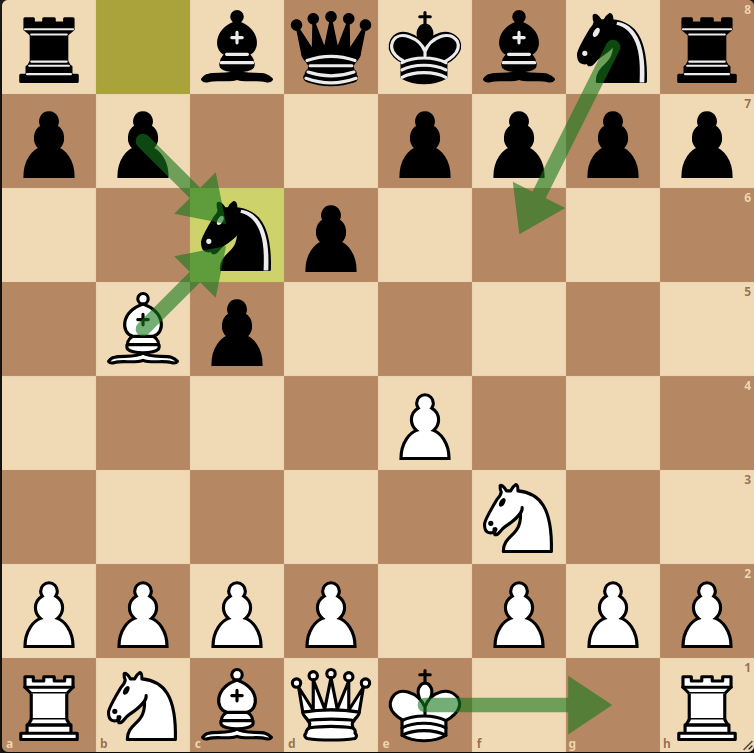
\includegraphics[width=\textwidth,height=6.0cm,keepaspectratio]{surlignage-coups}
\end{figure}


\section{Bibliographie}
 \bibliographystyle{plain}
 \bibliography{references}


\section{Besoins réalisés}
\label{Spec}

Voici la liste exhaustive des besoins qui ont été réalisés lors de ce projet. Pour chaque besoin, on retrouve une justification rapide de
pourquoi nous le considérons réalisé. Afin de visualiser au mieux les besoins, nous les avons présentés comme lors du premier rapport,
à l'exception que les sous-besoins précédemment identifiés n'y sont pas. Les encadrés bleus représentent les besoins fonctionnels et les
encadrés violets représentent les non-fonctionnels.

\begin{needbox}[F?: Titre]
    Template pour les besoins fonctionnels
    \begin{justificationbox}[Justification de réalisation]
        Explication justifiant la réalisation du besoin
    \end{justificationbox}
\end{needbox}

\begin{nonfunctionnalneedbox}[F?: Titre]
    Template pour les besoins non fonctionnels
    \begin{justificationbox}[Justification de réalisation]
        Explication justifiant la réalisation du besoin
    \end{justificationbox}
\end{nonfunctionnalneedbox}

\subsection{Généralités}

\begin{nonfunctionnalneedbox}[F1. Langage de programmation]
    Le langage de programmation du projet devra être Java et utiliser la spécification Java SE 17+.
    \begin{justificationbox}
        Le projet est développé en Java et respecte la spécification Java SE 17+.
    \end{justificationbox}
\end{nonfunctionnalneedbox}

\begin{nonfunctionnalneedbox}[F2: Style de codage]
    Le coding style du programme doit respecter le coding style de Google.
    \begin{justificationbox}
        Le coding style du Projet respecte le coding style de Google. Tous les commits ne le respectant pas
        ne sont pas acceptés sur GitLab. Pour s'en assurer, taper la commande mvn spotless:apply depuis
        chess/ et observer qu'aucun changement n'est appliqué.
    \end{justificationbox}
\end{nonfunctionnalneedbox}

\begin{nonfunctionnalneedbox}[F3: Langue par défaut dans le code]
    La documentation, le nom des variables, des fonctions et des fichiers devront être en anglais.
    \begin{justificationbox}
        Le code du projet a été écrit en anglais, qu'il s'agisse des noms de variables, de fonctions
        ou même de la documentation et des noms de fichiers/dossiers. 
    \end{justificationbox}
\end{nonfunctionnalneedbox}

\begin{nonfunctionnalneedbox}[F4. Système cible]
    Le programme devra fonctionner sur des systèmes d’exploitation GNU/Linux.
    \begin{justificationbox}
        COMPLETER.
    \end{justificationbox}
\end{nonfunctionnalneedbox}

\begin{nonfunctionnalneedbox}[F5. Documentation]
    Le programme et le code source devra être documenté : manuel utilisateur,
    option d’aide en ligne de commande et commentaires dans le code source.
    \begin{justificationbox}
        COMPLETER.
    \end{justificationbox}
\end{nonfunctionnalneedbox}

\begin{nonfunctionnalneedbox}[F6. Tests]
    Tester et valider le programme avec une couverture suffisante.
    \begin{justificationbox}
        COMPLETER.
    \end{justificationbox}
\end{nonfunctionnalneedbox}

\begin{nonfunctionnalneedbox}[F7: Bugs]
    Aucun bug menant à un crash ne doit être présent dans le programme. Les spécifications doivent être respectées
    et les erreurs doivent générer des messages d'erreur.
    \begin{justificationbox}
        COMPLETER.
    \end{justificationbox}
\end{nonfunctionnalneedbox}

\begin{nonfunctionnalneedbox}[F8: Performances]
    Evaluer des performances du programme de manière générale et pour différentes options et différentes configurations de jeu
    \begin{justificationbox}
        COMPLETER.
    \end{justificationbox}
\end{nonfunctionnalneedbox}

\begin{nonfunctionnalneedbox}[F9: Build-system]
    Établir un système de build pour le programme avec l'outil Maven pour Java. 
    \begin{justificationbox}
        Le projet se compile et utilise un système de build avec l'outil Maven.
    \end{justificationbox}
\end{nonfunctionnalneedbox}

\subsection{Bibliothèques et outils}

\begin{nonfunctionnalneedbox}[F10. Frameworks de test]
    Tester le code avec des frameworks donnés afin d'avoir un code sans bugs.
    \begin{justificationbox}
        Du Mock testing a été réalisé et le framework TestFX a notamment été utilisé.
    \end{justificationbox}
\end{nonfunctionnalneedbox}

\begin{nonfunctionnalneedbox}[F11. Gestion des options]
    La gestion des options sera basée sur la bibliothèque \textit{commons-cli}.
    \begin{justificationbox}
        COMPLETER.
    \end{justificationbox}
\end{nonfunctionnalneedbox}

\begin{nonfunctionnalneedbox}[F12: Bibliothèque graphique]
    La bibliothèque graphique utilisée sera basée sur JavaFx
    \begin{justificationbox}
        La partie Vue (frontend) se base sur le framework JavaFx.
    \end{justificationbox}
\end{nonfunctionnalneedbox}

\begin{nonfunctionnalneedbox}[F13: Internationalisation]
    Le framework d'internationalisation sera basé sur ResourcesBundle et Locale.
    \begin{justificationbox}
        COMPLETER.
    \end{justificationbox}
\end{nonfunctionnalneedbox}

\subsection{Options en ligne de commande}

\begin{nonfunctionnalneedbox}[F14. Nom de l’exécutable principal]
    L’exécutable principal doit s’appeler "chess" et permettre de lancer tout le programme.
    \begin{justificationbox}
        L’exécutable principal s’appele "chess" et permet de lancer tout le programme.
    \end{justificationbox}
\end{nonfunctionnalneedbox}

\begin{needbox}[F15. Usage général]
    \begin{justificationbox}
        COMPLETER.
    \end{justificationbox}
\end{needbox}

\begin{needbox}[F16: Aide en ligne de commande ]
    L'option '-h', '--help' affiche l'aide puis quitte.
    \begin{justificationbox}
        L’option ’-h’, ’–-help’ affiche l’aide puis quitte.
    \end{justificationbox}
\end{needbox}

\begin{needbox}[F17: Version ]
    L'option '-V', '--version' affiche la version puis quitte.
    \begin{justificationbox}
        L’option ’-V’, ’–-version’ affiche la version puis quitte.
    \end{justificationbox}
\end{needbox}

\begin{needbox}[F18: Mode verbose ]
    Réalisation d'un mode verbose, rapportant certaines informations supplémentaires au(x) joueur(s).
    \begin{justificationbox}
        L’option ’-v’, ’–-verbose’ permet d’afficher des
        informations supplémentaires pendant l’exécution.
    \end{justificationbox}
\end{needbox}
    
\begin{needbox}[F19: Mode debug ]
    Réalisation d'un mode debug, rapportant aux développeurs certaines informations sur le programme.
    \begin{justificationbox}
        L’option ’-d’, ’–-debug’ permet d’afficher des informations
        de débogage pendant l’exécution.
    \end{justificationbox}
\end{needbox}

\begin{needbox}[F20. Mode Blitz ]
    Permet de lancer le jeu en mode Blitz.
    \begin{justificationbox}
        L’option ’-b’, ’–-blitz’ permet de jouer en mode blitz.
        Dans ce mode, un temps limite est donné à chaque joueur
        pour jouer. Si le temps d’un des joueur est écoulé,
        il perd la partie.
    \end{justificationbox}
\end{needbox}

\begin{needbox}[F21. Durée du Blitz ]
    Permet de définir la durée du Blitz.
    \begin{justificationbox}
        COMPLETER.
    \end{justificationbox}
\end{needbox}

\begin{needbox}[F22: Mode \textit{Contest}]
    \begin{justificationbox}
        L’option ’-c FILENAME’, ’–-contest FILENAME’ permet de
        lancer le programme en mode ’contest’ en chargeant une
        partie depuis un fichier ’FILENAME’ (si fichier au bon format).
        Le programme affiche alors le joueur qui doit jouer ainsi que
        le coup à jouer.
    \end{justificationbox}
\end{needbox}

\begin{needbox}[F23: Mode IA ]
    Permet de lancer le programme en mode joueur artificiel.
    \begin{justificationbox}
        L’option ’-a[COLOR]’, ’–-ai[=COLOR]’ permet de lancer le
        programme en mode joueur artificiel avec la couleur COLOR
        (’W’, ’B’ et ’A’ (All), W par défaut).\\
        Note : en GUI, cliquer sur Menu 'Game' puis sur l'option 'Start'.
    \end{justificationbox}
\end{needbox}

\subsection{Interface utilisateur}

\begin{needbox}[F24. Interface en ligne de commande]
    \begin{justificationbox}
        Le programme posséde une interface en ligne de
        commande qui permet une interaction avec l’utilisateur via
        le terminal. Cette interface textuelle est lancée par défaut
        par le programme.
    \end{justificationbox}
\end{needbox}

\begin{needbox}[F25. Interface graphique]
    \begin{justificationbox}
        Le programme posséde une interface graphique qui
        permet les mêmes interactions que sur le CLI avec l’utilisateur
        via une fenêtre graphique. Cette interface graphique est
        lancée si l’option ’-g’, ’–-gui’ est donnée.
    \end{justificationbox}
\end{needbox}

\begin{needbox}[F26: Affichage de l'échiquier]
    À chaque coup, le programme devra afficher l'échiquier ainsi que le temps pris par chaque joueur si la partie est en blitz.
    \begin{justificationbox}
        À chaque coup, le programme affiche l’échiquier ainsi
        que le temps pris par chaque joueur si la partie est en blitz.
        Note: en ce qui concerne le temps pris par chaque joueur, le groupe
        a estimé plus logique d'afficher le temps pris sur toute la partie,
        pas le temps pris pour chaque coup.
    \end{justificationbox}
\end{needbox}

\begin{needbox}[F27: Notation des coups]
    Utilisation d'une notation codifiée pour les coups.
    \begin{justificationbox}
        COMPLETER.
    \end{justificationbox}
\end{needbox}

\begin{needbox}[F28: Représentation de l'historique]
    Afficher l'historique de la partie en indiquant le numéro de tour, le joueur, et le coup en notation algébrique.
    \begin{justificationbox}
        L’historique est représenté comme une liste des tours du
        jeu. Par exemple, le premier tour est affiché comme suit :
        ’1. B h4-h5 W e3-e5’ (le numéro du tour dans la partie, la
        couleur du joueur puis le coup en notation algébrique).
    \end{justificationbox}
\end{needbox}

\begin{needbox}[F29: En passant]
    Gestion du coup en passant des deux côtés.
    \begin{justificationbox}
        Le programme gère la prise en passant des deux côtés lorsque le coup est possible.
    \end{justificationbox}
\end{needbox}

\begin{needbox}[F30. Roque]
    Le jeu devra gérer le petit et grand roque des deux côtés.
    \begin{justificationbox}
        COMPLETER.
    \end{justificationbox}
\end{needbox}

\begin{needbox}[F31: Promotion du pion]
    Gérer la promotion du pion.
    \begin{justificationbox}
        Le programme gère la promotion du pion. Par défaut, pour l'IA,
        le pion se transforme en Dame.
    \end{justificationbox}
\end{needbox}

\begin{needbox}[F32: Abandon]
    Le programme devra permettre à un joueur d'abandonner la partie en cours de jeu.
    \begin{justificationbox}
        Le programme permet à un joueur d’abandonner
        la partie en cours de jeu s'il le souhaite.
    \end{justificationbox}
\end{needbox}

\begin{needbox}[F33: Affichage des messages]
    Le programme devra afficher des messages d'information
    pendant la partie en fonction du mode dans lequel il est
    (default, verbose, debug).
    \begin{justificationbox}
        Le programme affiche des messages d’information
        pendant la partie en fonction du mode dans lequel il est
        lancé (default, verbose, debug).
    \end{justificationbox}
\end{needbox}

\begin{needbox}[F34. Quitter et sauvegarder une partie]
    \begin{justificationbox}
        Le programme permet de quitter une partie en
        cours et de la sauvegarder dans un fichier.
        L'utilisateur choisit le nom du fichier.
    \end{justificationbox}
\end{needbox}

\begin{needbox}[F35. Sauvegarde de l’historique]
    \begin{justificationbox}
        Le programme peut sauvegarder l’historique des
        coups joués dans un fichier à la demande de l’utilisateur.
    \end{justificationbox}
\end{needbox}

\begin{needbox}[F36: Naviguer dans l'historique]
    Il doit être possible de revenir en arrière ou d'aller en avant dans l'historique des coups joués si tous les joueurs humains sont d'accord.
    \begin{justificationbox}
        Il est possible de revenir en arrière ("Undo") ou d’aller en avant
        ("Redo") dans l’historique des coups joués si tous les joueurs humains
        sont d’accord.
    \end{justificationbox}
\end{needbox}

\begin{needbox}[F37: Recommencer une partie]
    À tout moment, il doit être possible de recommencer une partie depuis le début en abandonnant la partie en cours.
    \begin{justificationbox}
        À tout moment, il est possible de recommencer une
        partie depuis le début en abandonnant la partie en cours.
    \end{justificationbox}
\end{needbox}

\begin{needbox}[F38: Fin de partie]
    Détecter la fin de la partie et déterminer le résultat en indiquant notamment qui est vainqueur (si vainqueur il y a).
    \begin{justificationbox}
        COMPLETER.
    \end{justificationbox}
\end{needbox}

\begin{needbox}[F39: Rejouer une partie]
    Possibilité de charger un fichier, naviguer dans l'historique et rejouer la partie depuis un coup choisi par l'utilisateur.
    \begin{justificationbox}
        L'utilisateur a la possibilité de charger une partie depuis un fichier,
        naviguer dans l'historique la partie et la reprendre depuis un certain
        coup. L'utilisateur doit demander la sauvegarde de cette nouvelle partie
        s'il souhaite ne pas la perdre.
    \end{justificationbox}
\end{needbox}

\subsection{Format d'entrée/sortie}

\begin{nonfunctionnalneedbox}[F40: Format de fichier simplifié]
    Permettre au joueur de sauvegarder et restaurer des fichires de jeu.
    \begin{justificationbox}
        COMPLETER.
    \end{justificationbox}
\end{nonfunctionnalneedbox}

\begin{nonfunctionnalneedbox}[F41: Format de l'historique]
    Lecture et écriture de l'historique de jeu.
    \begin{justificationbox}
        COMPLETER.
    \end{justificationbox}
\end{nonfunctionnalneedbox}

\begin{nonfunctionnalneedbox}[F42: Fichier de configuration]
    \begin{justificationbox}
        Le programme est capable de lire un fichier de
        configuration (.chessrc) qui contient les options par
        défaut du programme. Ce fichier est lu au démarrage du
        programme et les options qu’il contient sont utilisées par
        défaut.
    \end{justificationbox}
\end{nonfunctionnalneedbox}

\subsection{Structures internes}

\begin{needbox}[F43: Plateau de jeu]
    Les bitboards seront utilisées pour représenter l'état du plateau de jeu
    \begin{justificationbox}
        Des bitboards sont utilisés pour représenter l’état du plateau
        de jeu à chaque instant.
    \end{justificationbox}
\end{needbox}

\begin{needbox}[F44. Module bitboard]
    \begin{justificationbox}
        Un module bitboard rassemble les fonctions qui
        permettent de manipuler les bitboards.
    \end{justificationbox}
\end{needbox}

\begin{needbox}[F45. État du jeu]
    \begin{justificationbox}
        COMPLETER.
    \end{justificationbox}
\end{needbox}

\subsection{Interface graphique}

\begin{needbox}[F46: Fonctions de base]
    Possibilité d'utiliser les fonctions de base CLI directement depuis l'interface graphique.
    \begin{justificationbox}
        COMPLETER.
    \end{justificationbox}
\end{needbox}

\begin{needbox}[F47: Menu 'File']
    Menu principal 'File' permettant de gérer les fonctions liées aux parties.
    \begin{justificationbox}
        L’interface graphique comporte un menu principal
        avec les options (’New Game’), (’Load Game’),
        (’Save Game’), (’Quit’), (’Help’) et (’Settings’).
    \end{justificationbox}
\end{needbox}

\begin{needbox}[F48: Menu 'Game']
    Menu 'Game' permettant d'accéder à certaines options relatives à la partie.
    \begin{justificationbox}
        L’interface graphique comporte un menu de jeu qui
        permet de demander un conseil (’Hint’), naviguer dans
        l’historique (revenir en arrière, aller en avant, etc).
    \end{justificationbox}
\end{needbox}

\begin{needbox}[F49: Menu 'About']
    Menu 'About' permettant d'afficher quelques informations sur le Projet.
    \begin{justificationbox}
        L’interface graphique comporte un menu d’options 'About'
        qui permet de consulter des informations sur le programme
        (version, auteurs, ...).
    \end{justificationbox}
\end{needbox}

\begin{needbox}[F50: Affichage d'une partie en cours]
    Affiche le plateau courant et permet au joueur de bouger ses pièces.
    \begin{justificationbox}
        L’interface graphique affiche le plateau de jeu de la partie
        en cours ainsi que les informations habituellement présentes
        sur l’interface en ligne de commandes.
    \end{justificationbox}
\end{needbox}

\begin{needbox}[F51: Affichage des coups joués]
    Affiche l'historique des coups joués sur l'interface graphique.
    \begin{justificationbox}
        L’interface graphique affiche sur un côté de l’interface,
        les coups joués lors de la partie en les numérotant.
    \end{justificationbox}
\end{needbox}

\begin{needbox}[F52: Configuration d'une nouvelle partie]
    L'item 'New Game' du menu 'File' permettra de mener l'utilisateur à une fenêtre de configuration
    de la partie qui sera déjà remplie avec les paramètres par défaut. Qu'ils soient modifiés ou
    non, l'utilisateur pourra lancer la partie en cliquant sur 'Start'.
    \begin{justificationbox}
        Lorsque l'option 'New Game' est cliquée, l'utilisateur a le choix de lancer une nouvelle
        partie avec les paramètres par défaut, ou ajouter des paramètres. Un bouton 'Start Game'
        permet à l'utilisateur de lancer cette nouvelle partie.
    \end{justificationbox}
\end{needbox}

\subsection{Joueur artificiel}

\begin{needbox}[F53: Heuristique d'évaluation de position]
    Le programme devra comporter au moins une fonction
    capable de prendre un état du jeu et de lui donner un score en
    fonction de différents critères qui vous sembleront pertinents.
    \begin{justificationbox}
        Le programme comporte plusieurs fonctions capables de prendre
        un état du jeu et de lui donner un score en
        fonction de différents critères qui nous semblent pertinents.
    \end{justificationbox}
\end{needbox}

\begin{needbox}[F54. Algorithme de recherche Minimax]
    \begin{justificationbox}
        Le choix du meilleur coup se fait via une exploration
        de l’arbre des coups possibles via l’algorithme de recherche
        Minimax.
        Note: le groupe a préféré considérer AlphaBeta l'option
        par défaut car plus efficace donc ptentiellement mieux
        pourl'utilisateur (car plus de précision).
    \end{justificationbox}
\end{needbox}

\begin{needbox}[F55. AlphaBeta-pruning]
    \begin{justificationbox}
        Le choix du meilleur coup se fait via une exploration de
        l’arbre des coups possibles via l’algorithme de l'AlphaBeta-pruning.
        Cette option est activée par défaut si le programme est lancé
        en mode joueur artificiel.
        Néanmoins, l’option ’–-ai-mode ALPHA\_BETA’
    \end{justificationbox}
\end{needbox}

\begin{needbox}[F56: Monte Carlo Tree Search]
    \begin{justificationbox}
        L’option ’–-ai-mode mcts’ remplace l’algorithme d’exploration
        par défaut par un algorithme de Monte Carlo Tree Search (MCTS).
    \end{justificationbox}
\end{needbox}

\begin{needbox}[F57: Profondeur de recherche]
    \begin{justificationbox}
        L’option ’–-ai-depth DEPTH’ permet de spécifier la
        profondeur de recherche de l’algorithme de recherche.
        L’option ’–-ai-simulation SIMULATION permet de spécifier le
        nombre de simulations pour le recherche avec MCTS.
    \end{justificationbox}
\end{needbox}

\begin{needbox}[F58: Choix des heuristiques]
    \begin{justificationbox}
        Il est possible de gérer plusieurs heuristiques d’évaluation
        de position. L’option ’–-ai-heuristic HEURISTIC’
        permet de spécifier l’heuristique choisie parmi celles
        qui sont mises à disposition. Plusieurs peuvent être
        combinées (STANDARD défaut en utilise plusieurs).
    \end{justificationbox}
\end{needbox}

\begin{needbox}[F59: Heuristiques de fin de partie]
    \begin{justificationbox}
        Plusieurs heuristiques de fin de partie pour ont été créées
        afin d'optimiser l’évaluation des positions.
    \end{justificationbox}
\end{needbox}

\begin{needbox}[F60: Temps de réflexion borné]
    Permet de paramétrer la durée de "réflexion" de l'IA.
    \begin{justificationbox}
        L’option ’–-ai-time TIME’ permet de spécifier le temps
        de réflexion de l’algorithme de recherche. Si le temps est écoulé,
        le programme joue le meilleur coup trouvé jusqu’à présent.
        Par défaut, le temps de réflexion est de 5 secondes.
    \end{justificationbox}
\end{needbox}


\end{document}